\documentclass[12pt,letterpaper]{article}

\usepackage[utf8]{inputenc}
\usepackage[T1]{fontenc}
\usepackage[spanish,es-nodecimaldot,es-noshorthands]{babel}
\usepackage{lmodern}
\usepackage[top=2.5cm,bottom=2.5cm,left=3cm,right=2.5cm]{geometry}
\usepackage{graphicx}
\usepackage[dvipsnames,svgnames,x11names,table]{xcolor}
\usepackage[colorlinks=true,linkcolor=BrickRed,urlcolor=MidnightBlue,citecolor=ForestGreen]{hyperref}
\usepackage{amsmath,amssymb}
\usepackage{listings}
\usepackage[many,breakable,skins]{tcolorbox}
\usepackage{tikz}
\usepackage{pgfplots}
\usepackage{booktabs,longtable,array,tabularx,multirow,makecell}
\usepackage{fancyhdr}
\usepackage[explicit]{titlesec}
\usepackage{caption,subcaption}
\usepackage{enumitem}
\usepackage{mdframed}
\usepackage{microtype}
\usepackage{parskip}
\usepackage{float}
\usepackage{lastpage}
\usepackage{pdfpages}
\usepackage{fontawesome5}
\usetikzlibrary{shapes.geometric,arrows.meta,positioning,fit,backgrounds,
                decorations.pathreplacing,calc,matrix,shadows,
                shapes.multipart,shapes.symbols}
\pgfplotsset{compat=1.18}

% Color palette
\definecolor{catBase}{HTML}{1e1e2e}
\definecolor{catMantle}{HTML}{181825}
\definecolor{catBlue}{HTML}{89b4fa}
\definecolor{catGreen}{HTML}{a6e3a1}
\definecolor{catRed}{HTML}{f38ba8}
\definecolor{catYellow}{HTML}{f9e2af}
\definecolor{catMauve}{HTML}{cba6f7}
\definecolor{catText}{HTML}{cdd6f4}
\definecolor{catSurface}{HTML}{313244}
\definecolor{buapRed}{HTML}{8B0000}
\definecolor{buapGold}{HTML}{CFB53B}

% Page style
\pagestyle{fancy}
\fancyhf{}
\fancyhead[L]{}
\fancyhead[C]{\textit{Sistemas Operativos II --- Primavera 2026}}
\fancyhead[R]{\faUniversity\ Pág. \thepage/\pageref{LastPage}}
\renewcommand{\headrulewidth}{0.6pt}
\renewcommand{\footrulewidth}{0.4pt}
\setlength{\headheight}{15pt}

% Section formatting
\titleformat{\section}
  {\Large\bfseries\color{black}}
  {\color{buapGold}\(\blacksquare\) \thesection}{1em}{#1}
  [\vspace{0.5ex}{\color{buapRed}\titlerule[1pt]}]

\titleformat{\subsection}
  {\large\bfseries\color{MidnightBlue}}
  {\thesubsection}{1em}{#1}
  [\vspace{0.2ex}{\color{MidnightBlue}\rule{0.5\textwidth}{0.5pt}}]

\titleformat{\subsubsection}
  {\normalsize\bfseries\color{DarkSlateGray}}
  {\thesubsubsection}{1em}{#1}

% tcolorbox styles
\tcbset{
  codebox/.style={
    enhanced, breakable,
    colback=catBase, colframe=catBlue, coltext=catText,
    coltitle=catText, colbacktitle=catBlue,
    fonttitle=\ttfamily\bfseries,
    boxrule=0pt, leftrule=2pt, rightrule=2pt,
    arc=4pt, drop shadow,
    toptitle=1mm, bottomtitle=1mm
  },
  infobox/.style={
    enhanced, breakable,
    colback=Azure!10, colframe=MidnightBlue, coltext=black,
    coltitle=MidnightBlue, colbacktitle=Azure!10,
    fonttitle=\bfseries, title={\faInfoCircle\ #1},
    boxrule=0pt, leftrule=4pt, arc=0pt
  },
  alertbox/.style={
    enhanced, breakable,
    colback=catYellow!15, colframe=BrickRed, coltext=black,
    coltitle=BrickRed, colbacktitle=catYellow!15,
    fonttitle=\bfseries, title={\faExclamationTriangle\ #1},
    boxrule=0pt, leftrule=4pt, arc=0pt
  },
  successbox/.style={
    enhanced, breakable,
    colback=catGreen!10, colframe=ForestGreen, coltext=black,
    coltitle=ForestGreen, colbacktitle=catGreen!10,
    fonttitle=\bfseries, title={\faCheckCircle\ #1},
    boxrule=0pt, leftrule=4pt, arc=0pt
  },
  terminalbox/.style={
    enhanced, breakable,
    colback=catMantle, colframe=catSurface, coltext=catText,
    coltitle=catText, colbacktitle=catSurface,
    fonttitle=\ttfamily\bfseries, title={\faTerminal\ #1},
    fontupper=\ttfamily,
    boxrule=1pt, arc=0pt
  },
  screenshotbox/.style={
    enhanced, breakable,
    colback=gray!5, colframe=gray!70, coltext=black,
    fontupper=\small,
    boxrule=0.5pt, arc=4pt,
    drop shadow,
    titlerule=0pt,
    title={\faCamera\ \textbf{#1}},
    attach boxed title to top left={xshift=5mm,yshift=-2mm},
    boxed title style={empty, boxrule=0pt, colback=white, arc=0pt}
  }
}

% listings C++ config
\lstdefinestyle{cppstyle}{
  language=C++,
  basicstyle=\ttfamily\footnotesize\color{catText},
  keywordstyle=\color{catBlue}\bfseries,
  keywordstyle=[2]\color{catMauve},
  stringstyle=\color{catYellow},
  commentstyle=\color{gray}\itshape,
  numberstyle=\tiny\color{catYellow},
  numbers=left, numbersep=8pt,
  breaklines=true, tabsize=4,
  showstringspaces=false,
  frame=none,
  backgroundcolor={},
  morekeywords={size_t,uint32_t,optional,unique_ptr,shared_ptr,
                vector,deque,unordered_map,atomic,mutex,
                condition_variable,thread,lock_guard,unique_lock,
                PageID,FrameID,Process,Dispatcher,MemoryManager,
                HybridPolicy,ReplacementPolicy,ThreadPool,Frame,Page,Entry},
  morekeywords=[2]{std,chrono,this_thread}
}
\lstset{style=cppstyle}

\begin{document}

% COVER PAGE
\begin{titlepage}
\thispagestyle{empty}

\noindent
\begin{minipage}[c]{0.15\textwidth}
    
\includegraphics[width=\textwidth]{fcc_logo.png}
\end{minipage}
\hfill
\begin{minipage}[c]{0.65\textwidth}
    \centering
    {\Huge\bfseries\color{buapRed} Benemérita Universidad Autónoma de Puebla}\\[0.5cm]
    {\LARGE\bfseries\color{MidnightBlue} Facultad de Ciencias de la Computación}
\end{minipage}
\hfill
\begin{minipage}[c]{0.15\textwidth}
    
\includegraphics[width=\textwidth]{buap_logo.png}
\end{minipage}

\vspace{1cm}
{\color{buapRed}\rule{\textwidth}{2pt}}\vspace{1pt}
{\color{buapGold}\rule{\textwidth}{1pt}}

\begin{center}
    \vspace{2cm}
    {\Huge\bfseries\color{buapRed} Simulador de Administración de Memoria Virtual}\\[0.5cm]
    {\Large\bfseries\color{MidnightBlue} con Despacho de Procesos, Arquitectura Cliente-Servidor y Balanceo de Carga mediante Thread Pool}

    \vspace{0.5cm}
    {\large\textbf{Curso:} Sistemas Operativos II}\\[0.2cm]
    {\large\textbf{Profesora:} Dra. Hilda Castillo Zacatelco}\\[0.2cm]
    {\large\textbf{Semestre:} Primavera 2026}
    \vspace{0.5cm}

    \renewcommand{\arraystretch}{1.5}
    \begin{tabular}{l}
        \toprule
        \textbf{Nombre} \\
        \midrule
        Razo Montañez Gael Askary \\
        Ángel Hernández González \\
        José Gabriel Hernández Mejía \\
        \bottomrule
    \end{tabular}

    \vfill
    {\color{buapGold}\rule{\textwidth}{1pt}}\vspace{1pt}
    {\color{buapRed}\rule{\textwidth}{2pt}}\vspace{0.2cm}
    {\large Mayo 2026}
\end{center}
\end{titlepage}

\newpage
\tableofcontents
\newpage
\listoffigures
\newpage
\listoftables
\newpage

\section{Introducción}

El diseño de los sistemas operativos modernos está intrínsecamente ligado al manejo eficiente de la jerarquía de memoria. En sistemas multiprogramados, la memoria principal (RAM) es un recurso limitado y compartido que debe ser protegido y administrado cuidadosamente para asegurar la estabilidad del sistema. La memoria virtual surge como una solución elegante a este problema, proveyendo a cada proceso la ilusión de poseer un espacio de direcciones grande y contiguo, aislado del resto de los procesos y de la ubicación física real de los datos. La paginación es el mecanismo dominante de memoria virtual en las arquitecturas contemporáneas, como x86-64. Al dividir la memoria en bloques de tamaño fijo (páginas lógicas y marcos físicos), el sistema operativo simplifica la asignación y elimina la fragmentación externa. Sin embargo, dado que el espacio de direcciones virtuales supera con creces la capacidad de la memoria física, es inevitable que ocurran fallos de página. Un fallo de página obliga al sistema a suspender el proceso, acceder al disco (un dispositivo de almacenamiento secundario significativamente más lento) y cargar la página requerida en un marco físico. Cuando la RAM está llena, el sistema operativo debe decidir qué marco liberar para dar cabida a la nueva página. Esta decisión es gobernada por el algoritmo de reemplazo de páginas. Una elección deficiente puede llevar a la expulsión de una página que será requerida inmediatamente, provocando una avalancha de fallos de página que degrada severamente el rendimiento del sistema, un fenómeno conocido como \textit{thrashing}. La teoría del conjunto de trabajo (working set) establece que los algoritmos de reemplazo deben retener en memoria aquellas páginas que el proceso necesita activamente, adaptándose a los cambios de localidad de referencia a lo largo del tiempo. El objetivo principal de este proyecto es desarrollar un simulador pedagógico paso a paso que exponga de manera transparente todo el estado interno de la administración de memoria virtual. A diferencia de un kernel real, donde estas estructuras están ocultas, este simulador permite visualizar el estado de la tabla de páginas, la matriz de memoria física y las listas de la política de reemplazo en tiempo real. Además, para dotar al proyecto de relevancia industrial y conectarlo con los paradigmas actuales de concurrencia y redes, el simulador ha sido extendido con una arquitectura cliente-servidor basada en sockets TCP. En lugar de un modelo ingenuo de un hilo por cliente, se ha implementado un mecanismo de balanceo de carga mediante un \textit{Thread Pool}. Esta arquitectura no solo optimiza el uso de recursos del sistema anfitrión, sino que simula un entorno de procesamiento por lotes concurrente donde múltiples procesos de diferentes usuarios compiten por los recursos de la CPU y la memoria. En los siguientes capítulos, este documento desglosará el marco teórico subyacente (Capítulo 2), la arquitectura y diseño del sistema (Capítulo 3), los detalles críticos de la implementación en C++20 (Capítulo 4), el manual técnico para desarrolladores (Capítulo 5), la guía de uso de la interfaz gráfica y de línea de comandos (Capítulo 6), los resultados de las pruebas de estrés (Capítulo 7), y finalmente una discusión y conclusión sobre los aprendizajes obtenidos. \newpage
\section{Marco Teórico}

\subsection{Memoria Virtual y Paginación}

La memoria virtual abstrae la memoria principal de un dispositivo de almacenamiento masivo, típicamente un disco duro o SSD. La unidad fundamental de este esquema es la \textit{página}, un bloque contiguo de memoria, usualmente de 4 KB. Las direcciones generadas por la CPU son direcciones lógicas (o virtuales), las cuales deben ser traducidas a direcciones físicas por una unidad de hardware llamada MMU (Memory Management Unit). La traducción se realiza mediante una estructura de datos mantenida por el sistema operativo denominada \textit{Tabla de Páginas}. Para acelerar este proceso, la MMU cuenta con una caché de traducciones conocida como TLB (Translation Lookaside Buffer). Cada entrada de la tabla de páginas (PTE) no solo contiene el número de marco físico correspondiente, sino también bits de control como el bit de validez (indica si la página está en RAM), el bit de modificación o sucio (indica si la página ha sido escrita y requiere guardarse en disco) y los bits de protección (lectura, escritura, ejecución). \begin{figure}[H]
\centering
\begin{tikzpicture}[
    node distance=0cm,
    font=\small,
    box/.style={draw, rectangle, minimum height=1cm, align=center, outer sep=0pt},
    arrow/.style={-{Stealth}, thick}
]
    % Logical Address
    \node[box, fill=catBlue!20, minimum width=2.2cm] (log_p) {Página ($p$)};
    \node[box, fill=catGreen!20, minimum width=2.2cm, right=of log_p] (log_d) {Despl. ($d$)};
    \node[above=0.2cm of log_p.north east] {\textbf{Dirección Lógica}};

    % Page Table
    \matrix[matrix of nodes, nodes={draw, minimum width=2.5cm, minimum height=0.6cm}, row sep=-\pgflinewidth, right=1.5cm of log_d] (pt) {
        Marco 0 \\
        ... \\
        |[fill=catYellow!40, font=\bfseries]| Marco $F$ \\
        ... \\
        Marco $N$ \\
    };
    \node[above=0.2cm of pt.north] {\textbf{Tabla de Páginas}};

    % Physical Address
    \node[box, fill=catYellow!40, minimum width=2.2cm, right=1.5cm of pt] (phys_f) {Marco ($F$)};
    \node[box, fill=catGreen!20, minimum width=2.2cm, right=of phys_f] (phys_d) {Despl. ($d$)};
    \node[above=0.2cm of phys_f.north east] {\textbf{Dirección Física}};

    % Arrows
    \draw[arrow] (log_p.south) -- ++(0,-0.6) -| ([xshift=-0.3cm]pt-3-1.west) |- (pt-3-1.west);
    \draw[arrow] (pt-3-1.east) -- (phys_f.west);
    \draw[arrow] (log_d.south) -- ++(0,-1.2) -| (phys_d.south);
\end{tikzpicture}
\caption{Proceso de traducción de direcciones lógicas a físicas mediante paginación.}
\label{fig:traduccion}
\end{figure}

\subsection{Fallos de Página}

Un fallo de página ocurre cuando la MMU intenta traducir una dirección lógica cuya entrada en la tabla de páginas tiene el bit de validez en cero, indicando que la página reside en disco. Esto genera un \textit{trap} al sistema operativo.

\begin{figure}[H]
\centering
\begin{tikzpicture}[
    node distance=1cm and 1cm,
    font=\footnotesize,
    action/.style={draw, rectangle, rounded corners, fill=catBlue!10, text width=2.5cm, align=center, minimum height=1cm},
    decision/.style={draw, diamond, fill=catYellow!20, text width=2cm, align=center, inner sep=0pt},
    arrow/.style={-{Stealth}, thick}
]
    \node[action] (start) {Acceso a CPU};
    \node[action, right=of start] (mmu) {MMU consulta Tabla};
    \node[decision, right=of mmu] (valid) {¿Bit válido = 1?};
    \node[action, fill=catGreen!20, right=of valid, text width=1.5cm] (hit) {HIT\\Retornar};

    \node[action, below=of valid] (trap) {Trap al OS};
    \node[decision, below=of trap] (free) {¿Marco libre?};

    \node[action, right=of free] (load1) {Cargar pág. en marco libre};
    \node[action, left=of free] (algo) {Ejecutar Alg. Reemplazo};
    \node[decision, below=of algo] (dirty) {¿Página víctima sucia?};
    \node[action, left=of dirty] (write) {Escribir víctima a disco};
    \node[action, below=of dirty] (load2) {Cargar pág. en marco víctima};
    \node[action, below=of load1] (update) {Actualizar Tabla};

    \draw[arrow] (start) -- (mmu);
    \draw[arrow] (mmu) -- (valid);
    \draw[arrow] (valid) -- node[above] {Sí} (hit);
    \draw[arrow] (valid) -- node[right] {No} (trap);
    \draw[arrow] (trap) -- (free);

    \draw[arrow] (free) -- node[above] {Sí} (load1);
    \draw[arrow] (free) -- node[above] {No} (algo);

    \draw[arrow] (algo) -- (dirty);
    \draw[arrow] (dirty) -- node[above] {Sí} (write);
    \draw[arrow] (write) |- (load2);
    \draw[arrow] (dirty) -- node[right] {No} (load2);

    \draw[arrow] (load1) -- (update);
    \draw[arrow] (load2) -| (update);
\end{tikzpicture}
\caption{Diagrama de flujo del manejador de fallos de página.}
\label{fig:pagefault}
\end{figure}

\subsection{Algoritmos de Reemplazo}

\subsubsection{FIFO}
El reemplazo FIFO (First-In, First-Out) expulsa la página que lleva más tiempo en memoria. Aunque es simple, sufre de la anomalía de Bélády: aumentar el número de marcos de RAM puede \textit{aumentar} el número de fallos de página. \subsubsection{LRU (Least Recently Used)}
LRU expulsa la página que no ha sido accedida por más tiempo. Es libre de anomalías y aproxima bien el principio de localidad. Sin embargo, su implementación exacta (usando pilas o marcas de tiempo en cada acceso) requiere soporte extenso de hardware y es costosa. \subsubsection{Clock (Segunda Oportunidad)}
Aproxima LRU usando un bit de referencia en la tabla de páginas. Una manecilla recorre los marcos; si el bit es 1, le da una "segunda oportunidad" (lo pone en 0) y avanza. Si es 0, lo reemplaza. Es eficiente y fácil de implementar. \subsubsection{ARC (Adaptive Replacement Cache)}
ARC mantiene dos listas principales: T1 (recientemente accedidas, localidad de recencia) y T2 (frecuentemente accedidas, localidad de frecuencia), junto con historiales fantasma B1 y B2 para las páginas expulsadas. ARC adapta dinámicamente un parámetro $p$ (tamaño objetivo de T1) según los hits en B1 o B2. \subsubsection{CAR (Clock with Adaptive Replacement)}
CAR es el algoritmo implementado en la política híbrida del simulador. Combina la adaptabilidad de ARC con la eficiencia de Clock. En lugar de mantener listas LRU exactas para T1 y T2, CAR utiliza manecillas de reloj sobre listas circulares, obteniendo un costo de selección de víctima amortizado de $\mathcal{O}(1)$, manteniendo la resistencia al thrashing y la adaptación entre frecuencia y recencia. \subsubsection{Comparación de Algoritmos}

\begin{table}[H]
\centering
\rowcolors{2}{catBlue!10}{white}
\begin{tabular}{@{}llcccc@{}}
\toprule
\rowcolor{catBlue!40}
\textbf{Algoritmo} & \textbf{Complejidad} & \textbf{Sin Bélády} & \textbf{Frecuencia} & \textbf{Adaptativo} & \textbf{Costo Impl.} \\ \midrule
FIFO  & $\mathcal{O}(1)$ & No & No & No & Bajo \\
LRU   & $\mathcal{O}(1)$ (hardware) & Sí & No & No & Alto \\
Clock & $\mathcal{O}(1)$ amortizado & No & No & No & Bajo \\
ARC   & $\mathcal{O}(1)$ amortizado & Sí & Sí & Sí & Medio-Alto \\
CAR   & $\mathcal{O}(1)$ amortizado & Sí & Sí & Sí & Medio \\ \bottomrule
\end{tabular}
\caption{Comparación de algoritmos de reemplazo de páginas.}
\label{tab:alg_comp}
\end{table}

\subsection{Despacho --- Round Robin}
Round Robin asigna la CPU a cada proceso
por un tiempo fijo llamado quantum ($q$).
Las fórmulas fundamentales son:
\begin{itemize}
    \item Tiempo de retorno (Turnaround): $T_r = T_f - T_a$ (Tiempo final - Tiempo de llegada)
    \item Tiempo de espera: $T_w = T_r - T_{burst}$
\end{itemize}

Ejemplo: 3 procesos con ráfagas y un $q=5$.
\begin{figure}[H]
\centering
\begin{tikzpicture}
    % Axis
    \draw[->, thick] (0,0) -- (12,0) node[right] {Tiempo};
    \foreach \x in {0,2,4,6,8,10} {
        \draw (\x, 0.1) -- (\x, -0.1) node[below] {\x};
}
    % Bars
    \draw[fill=catBlue!50, draw=catBlue!80, thick] (0, 0.5) rectangle (4, 1.5) node[midway, black] {P1};
    \draw[fill=catGreen!50, draw=catGreen!80, thick] (4, 0.5) rectangle (8, 1.5) node[midway, black] {P2};
    \draw[fill=catYellow!50, draw=catYellow!80, thick] (8, 0.5) rectangle (10, 1.5) node[midway, black] {P3};
\end{tikzpicture}
\caption{Diagrama de Gantt mostrando un despacho Round Robin simplificado.}
\end{figure}

\subsection{Programación Concurrente --- Thread Pool}
El patrón \textit{Thread Pool} mantiene un conjunto fijo de hilos trabajadores que consumen tareas de una cola compartida. Se protege la cola mediante un \texttt{std::mutex} y se señaliza la disponibilidad de tareas mediante \texttt{std::condition\_variable}. Este modelo previene la explosión de hilos (thread explosion) y el sobrecosto de cambios de contexto asociado a crear un hilo por cada conexión TCP entrante, permitiendo escalar a miles de conexiones usando un número constante de hilos igual al número de núcleos físicos de la CPU. Para evitar la inversión de prioridad, hilos de mantenimiento (como el \textit{stepper} de simulación) pueden usar \texttt{std::try\_to\_lock}. \subsection{Arquitectura Cliente-Servidor TCP}

\begin{figure}[H]
\centering
\begin{tikzpicture}[
    node distance=1.5cm,
    font=\small,
    lifeline/.style={draw, thick, minimum height=6cm},
    arrow/.style={-{Stealth}, thick}
]
    \node (client_title) at (0, 0) {\textbf{Cliente}};
    \node (server_title) at (6, 0) {\textbf{Servidor}};

    \draw[thick] (0, -0.5) -- (0, -6.5);
    \draw[thick] (6, -0.5) -- (6, -6.5);
    \draw[arrow] (-1, -1) -- node[above] {socket() + connect()} (0, -1);
    \draw[arrow] (7, -1) -- node[above] {bind() + listen() + accept()} (6, -1);
    \draw[arrow] (0, -2) -- node[above] {CREATE <pid> ...} (6, -2);
    \draw[arrow, dashed] (6, -3) -- node[above] {OK <pid>} (0, -3);
    \node at (3, -4) {\textit{(El despachador simula el proceso)}};

    \draw[arrow, dashed] (6, -5) -- node[above] {DONE <pid> ...} (0, -5);
    \draw[arrow] (0, -6) -- node[left] {close()} (0, -6.5);
    \draw[arrow] (6, -6) -- node[right] {close()} (6, -6.5);
\end{tikzpicture}
\caption{Diagrama de secuencia de la interacción cliente-servidor mediante sockets TCP.}
\label{fig:tcp_seq}
\end{figure}\newpage
\section{Diseño del Sistema}

\subsection{Visión General de la Arquitectura}

\begin{figure}[H]
\centering
\begin{tikzpicture}[
    node distance=1cm and 0.8cm,
    font=\footnotesize,
    box/.style={draw, rectangle, rounded corners, minimum height=1cm, minimum width=2.5cm, align=center, fill=catBlue!10},
    arrow/.style={-{Stealth}, thick}
]
    \node[box] (mm) {MemoryManager};
    \node[box, right=of mm] (disp) {Dispatcher};
    \node[box, right=of disp] (policy) {HybridPolicy (CAR)};
    \node[box, right=0.8cm of policy, fill=catYellow!20] (client) {Client CLI};

    \node[box, below=1cm of disp] (proc) {Process};

    \node[box, above=2.2cm of mm] (gui) {MainWindow\\(Qt6 GUI)};
    \node[box, above=2.2cm of client] (server) {Server + ThreadPool\\+ Monitor};

    % Línea divisoria ajustada para no desbordar el margen derecho
    \draw[dashed, color=gray]
        ([xshift=-0.5cm,yshift=1.1cm]mm.north west) --
        ([xshift=0.5cm,yshift=1.1cm]client.north east)
        node[above left, text=black] {API Interna (C++20)};

    \draw[<->, thick] (mm) -- (disp);
    \draw[<->, thick] (disp) -- (policy);
    \draw[arrow] (proc) -- (disp);

    % Etiqueta TCP con fondo blanco para que la línea gris no la cruce
    \draw[<->, thick, dashed] (client) -- node[fill=white, inner sep=3pt, text=black] {TCP} (server);

    % Indicador de ThreadPool
    \node[draw, dashed, fit=(server), inner sep=0.3cm, label=above:ThreadPool] {};
\end{tikzpicture}
\caption{Arquitectura de dos capas del simulador MemManager.}
\end{figure}

\subsection{Diagrama de Clases Completo}

\begin{figure}[H]
\centering
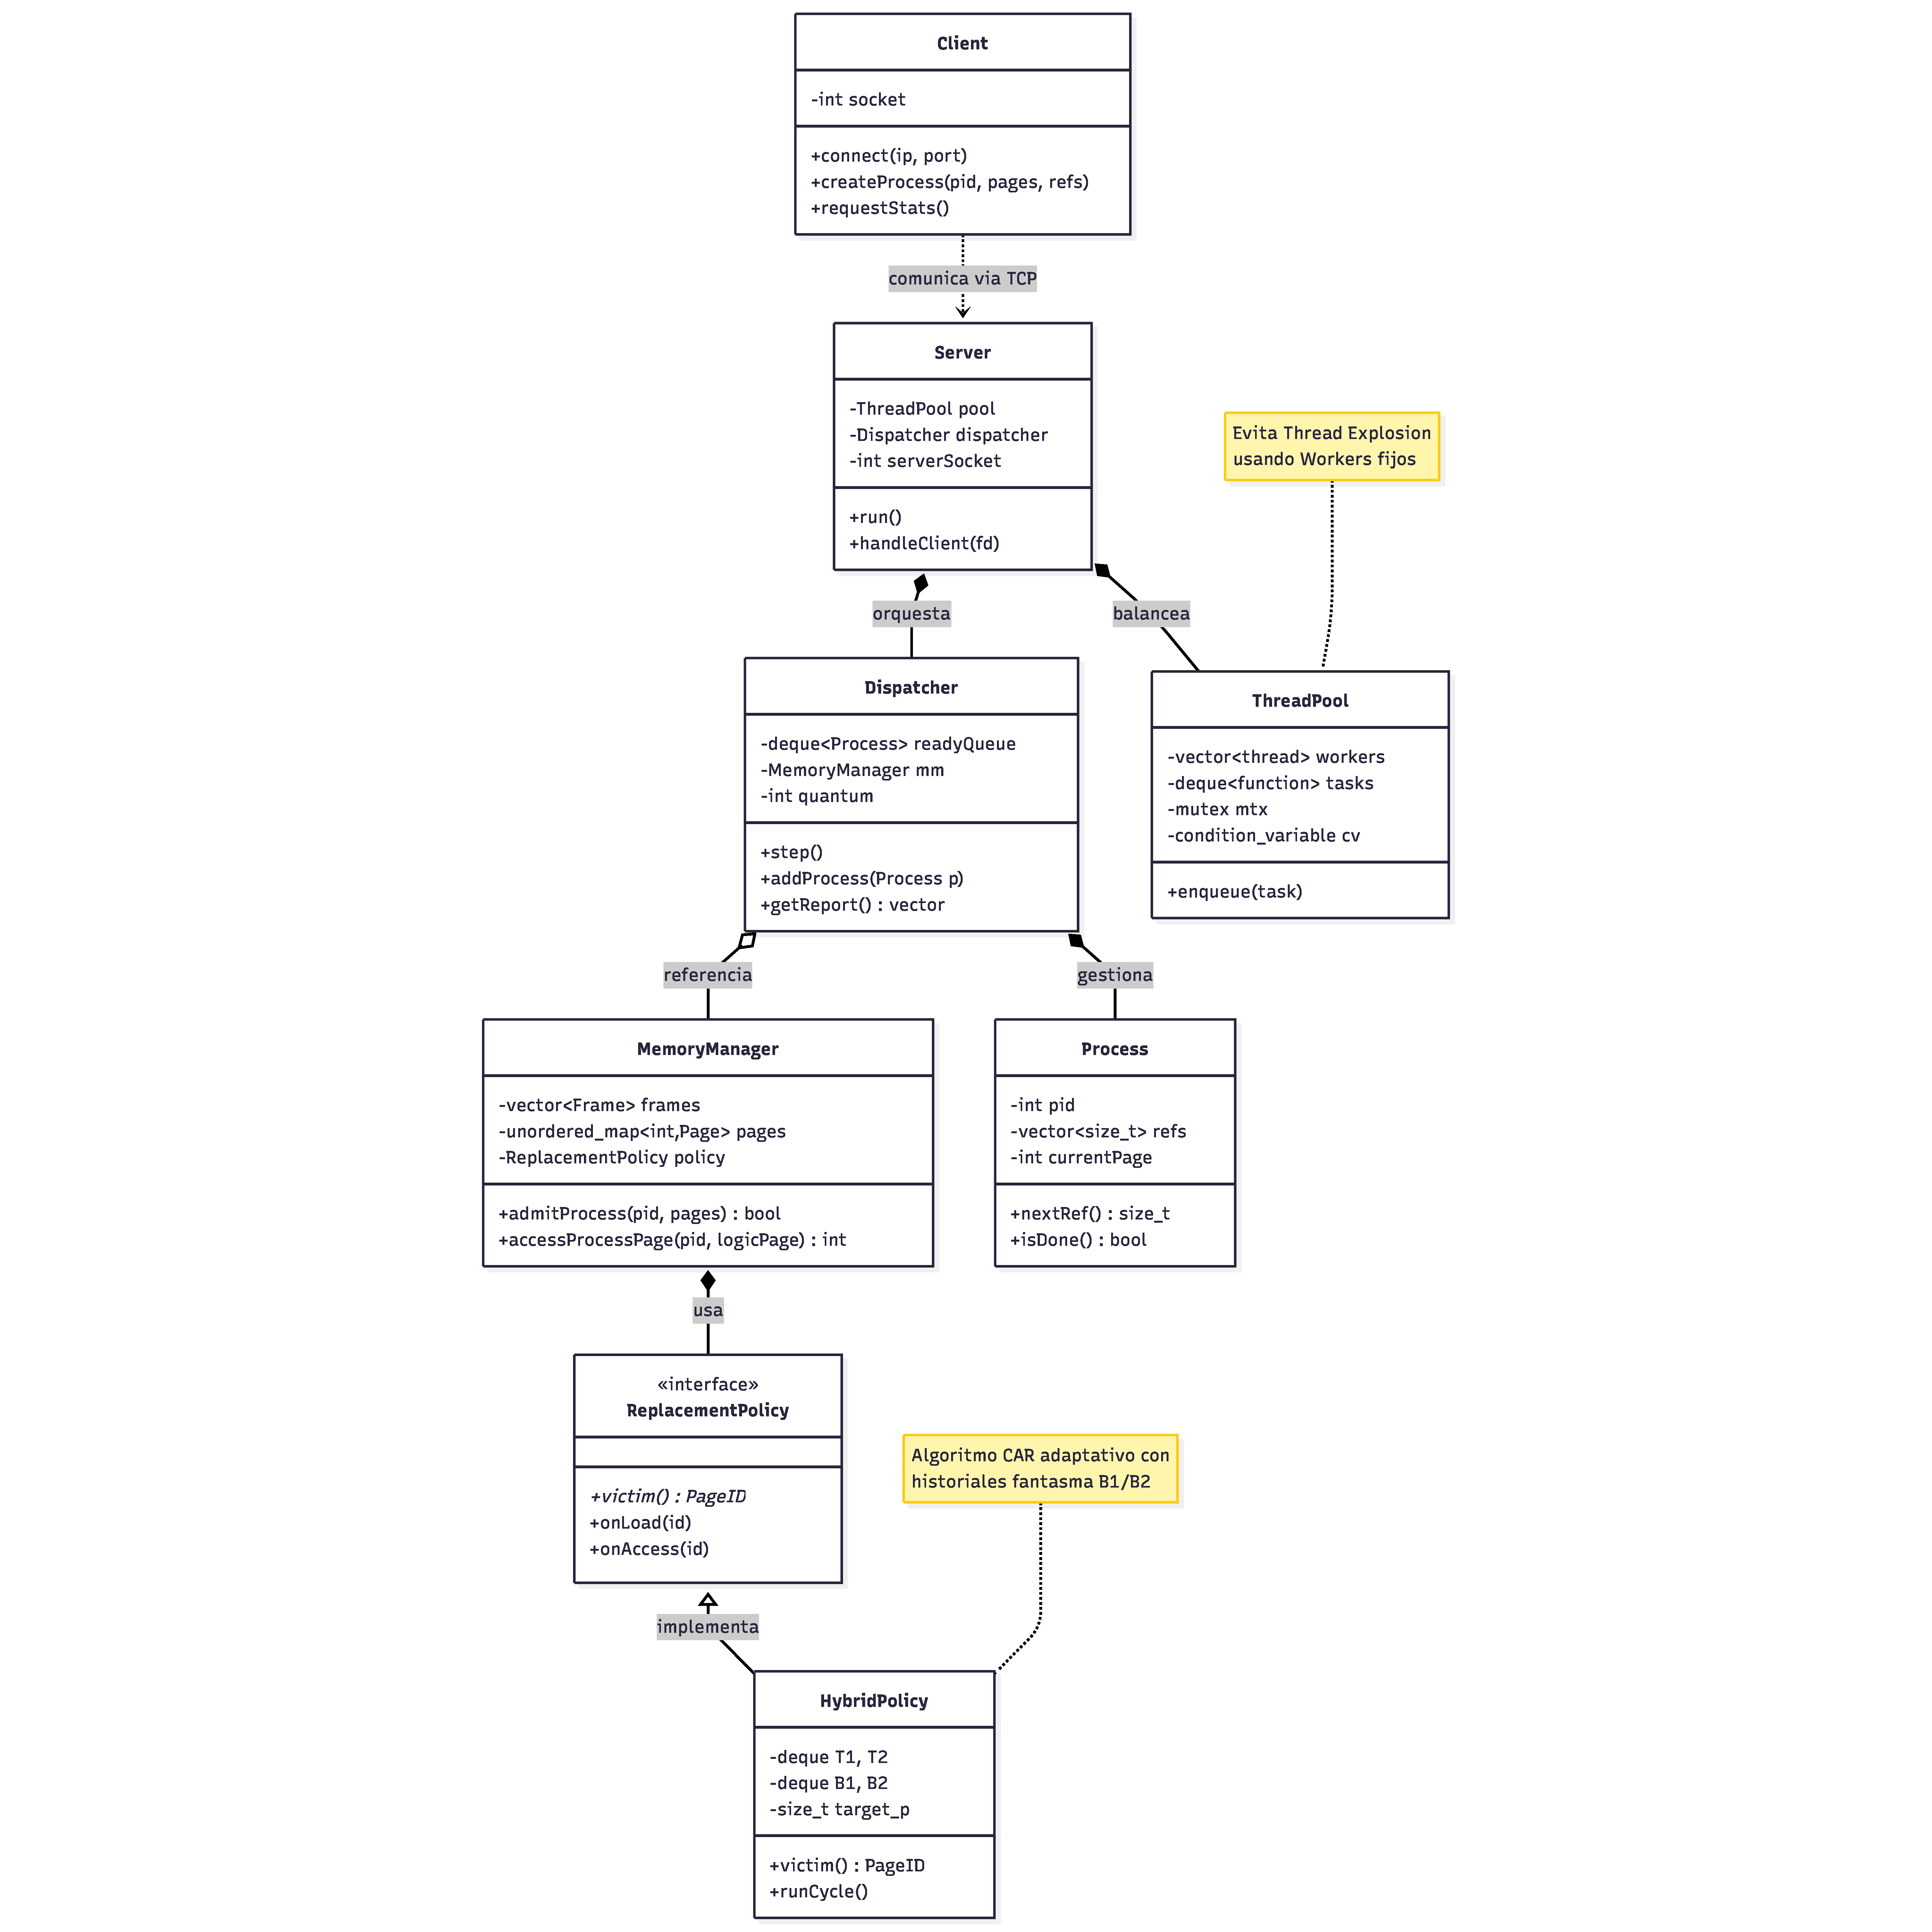
\includegraphics[width=\textwidth]{UML_Memmanager.pdf}
\caption{Diagrama de clases UML del núcleo del simulador.}
\end{figure}

\subsection{HybridPolicy --- Diseño Detallado}

La clase \texttt{HybridPolicy} implementa el algoritmo CAR, utilizando cuatro estructuras de datos:
\begin{itemize}
    \item \textbf{T1}: Una \texttt{std::deque} de entradas (ID de página y bit de referencia R).
Mantiene páginas recientemente cargadas (vistas una vez).
    \item \textbf{T2}: Una \texttt{std::deque} de entradas. Mantiene páginas frecuentemente accedidas (vistas múltiples veces).
\item \textbf{B1}: Un historial fantasma (solo IDs) de páginas expulsadas de T1.
\item \textbf{B2}: Un historial fantasma de páginas expulsadas de T2.
    \item \textbf{p\_}: El tamaño objetivo de T1.
Se adapta dinámicamente: aumenta si hay un hit en B1, disminuye si hay un hit en B2.
\end{itemize}

\begin{figure}[H]
\centering
\begin{tikzpicture}[
    node distance=2.5cm and 3cm,
    font=\scriptsize,
    state/.style={draw, rectangle, rounded corners, minimum width=2.2cm, minimum height=1cm, align=center, fill=catBlue!10},
    arrow/.style={-{Stealth}, thick}
]
    \node[state] (new) {Nueva página};
    \node[state, right=of new] (load) {onLoad()};
    \node[state, above right=of load, yshift=1cm] (t2) {T2 (Frecuente)};
    \node[state, below right=of load, yshift=-1cm] (t1) {T1 (Reciente)};
    \node[state, right=of t2] (b2) {B2 (Fantasma)};
    \node[state, right=of t1] (b1) {B1 (Fantasma)};

    \draw[arrow] (new) -- (load);
    \draw[arrow] (load) -- node[above, sloped, yshift=0.1cm] {Hit en B1/B2?} (t2);
    \draw[arrow] (load) -- node[below, sloped, yshift=-0.1cm] {Miss total} (t1);
    \draw[arrow] (t1) -- node[right, align=center] {onAccess(R=1)} (t2);
    \draw[arrow] (t2) edge[loop above] node {onAccess(R=1)} (t2);
    \draw[arrow] (t1) -- node[below] {victim() (R=0)} (b1);
    \draw[arrow] (t2) -- node[above] {victim() (R=0)} (b2);
    \draw[arrow, dashed] (b1) to[bend left=55] node[above, align=center, pos=0.6] {Hit futuro \\ $\rightarrow$ Aumenta $p$} (load);
    \draw[arrow, dashed] (b2) to[bend right=55] node[below, align=center, pos=0.6] {Hit futuro \\ $\rightarrow$ Disminuye $p$} (load);
\end{tikzpicture}
\caption{Máquina de estados de la política de reemplazo híbrida CAR.}
\end{figure}

Para simular el barrido de la manecilla de reloj (Clock) sin necesidad de recorrer explícitamente listas enlazadas en cada acceso, la \texttt{HybridPolicy} incorpora un método \texttt{runCycle()}.
Cada \texttt{REFS\_PER\_CYCLE} (por defecto 3 referencias de memoria gestionadas por el \texttt{MemoryManager}), se ejecuta un "tick" del reloj que limpia todos los bits R (los pone en \texttt{false}) en T1 y T2.
Esta aproximación mantiene el costo temporal por referencia estrictamente acotado, aliviando el simulador de iteraciones costosas sobre colecciones largas.
\subsection{MemoryManager --- Modelo de Dos Niveles}

El \texttt{MemoryManager} gestiona el espacio de direcciones con dos mapas de bits principales: \texttt{bitmap\_} (páginas virtuales asignadas) y \texttt{inRam\_} (páginas residentes en memoria física).
\begin{figure}[H]
\centering
\begin{tikzpicture}[
    font=\footnotesize,
    cell/.style={draw, rectangle, minimum width=0.5cm, minimum height=0.5cm, inner sep=0pt},
    arrow/.style={-{Stealth}, thick, color=MidnightBlue}
]
    \node at (-1.5, 1) {Espacio Virtual};
    \foreach \x in {0,...,15} {
        \ifnum\x=2 \node[cell, fill=catBlue!50] (v\x) at (\x*0.5, 1) {};
\else\ifnum\x=5 \node[cell, fill=catGreen!50] (v\x) at (\x*0.5, 1) {};
        \else\ifnum\x=12 \node[cell, fill=catYellow!50] (v\x) at (\x*0.5, 1) {};
\else \node[cell, fill=gray!20] (v\x) at (\x*0.5, 1) {}; \fi\fi\fi
    }
    \node at (8.5, 1) {... 255};
    \node at (-1.5, -0.5) {Marcos RAM};
    \foreach \x in {0,...,7} {
        \ifnum\x=1 \node[cell, fill=catGreen!50] (r\x) at (\x*0.5+2, -0.5) {};
\else\ifnum\x=3 \node[cell, fill=catBlue!50] (r\x) at (\x*0.5+2, -0.5) {};
        \else \node[cell, fill=white] (r\x) at (\x*0.5+2, -0.5) {};
\fi\fi
    }
    \node at (6.5, -0.5) {... 15};

    \draw[arrow] (r1.north) -- (v5.south);
    \draw[arrow] (r3.north) -- (v2.south);

    \node at (4, -1.5) {\textit{Las páginas no apuntadas están en Disco (Swap)}};
\end{tikzpicture}
\caption{Mapeo de memoria virtual a memoria física mediante la tabla global de marcos.}
\end{figure}\subsection{Dispatcher --- Round Robin con String de Referencias}

El despachador es responsable de ejecutar el algoritmo Round Robin simulado.
En lugar de ráfagas de tiempo abstracto, el despachador consume una lista determinista de accesos a memoria (string de referencias) por cada proceso.
Cada llamada a \texttt{step()}:
\begin{enumerate}
    \item Selecciona el proceso activo de la cola \texttt{readyQueue\_}.
    \item Llama a \texttt{nextRef()} para obtener la siguiente página lógica a acceder.
    \item Manda a llamar a \texttt{mm\_.accessProcessPage(pid, logicalPage)}.
    \item Registra el resultado: hit, fallo suave, o fallo duro (que incrementa \texttt{pageFaults\_}).
    \item Incrementa el tiempo de la simulación y el \texttt{quantumUsed\_}.
    \item Si el quantum se agota o el proceso termina, invoca \texttt{rotateProcess()}.
\end{enumerate}

\begin{table}[H]
\centering
\rowcolors{2}{catBlue!10}{white}
\begin{tabular}{@{}lll@{}}
\toprule
\rowcolor{catBlue!40}
\textbf{Condición} & \textbf{Acción} & \textbf{Estado Siguiente} \\ \midrule
Quantum agotado & \texttt{rotateProcess()} & Proceso al final de \texttt{readyQueue\_} \\
Proceso terminó refs.
& Generar reporte & Proceso removido de \texttt{readyQueue\_} \\
Fallo de página & Bloqueo / I/O simulado & \textit{Implementado de forma simplificada} \\ \bottomrule
\end{tabular}
\caption{Transiciones de estado del Dispatcher.}
\end{table}

\subsection{Thread Pool --- Diseño Detallado}

\begin{figure}[H]
\centering
\begin{tikzpicture}[
    node distance=1.5cm,
    font=\footnotesize,
    box/.style={draw, rectangle, rounded corners, minimum height=1cm, minimum width=2.5cm, align=center, fill=catBlue!10},
    qbox/.style={draw, rectangle, minimum height=1cm, minimum width=1.5cm, align=center, fill=catYellow!20},
    worker/.style={draw, rectangle, rounded corners, minimum height=0.8cm, minimum width=2cm, align=center, fill=catGreen!10},
    arrow/.style={-{Stealth}, thick}
]

    \node (clients) at (-2, 0) {\textbf{Clientes}};
    \node[box, right=1.5cm of clients] (accept) {Accept\\Loop};

    \draw[arrow] ([yshift=0.2cm]clients.east) -- ([yshift=0.2cm]accept.west);
    \draw[arrow] (clients.east) -- (accept.west);
    \draw[arrow] ([yshift=-0.2cm]clients.east) -- ([yshift=-0.2cm]accept.west);

    \node[qbox, right=1.5cm of accept] (queue) {Cola de\\Tareas};
    \draw[arrow] (accept) -- node[above] {\texttt{enqueue()}} (queue);
    \node[worker, right=2cm of queue, yshift=1.5cm] (w1) {Worker 1};
    \node[worker, right=2cm of queue, yshift=0.5cm] (w2) {Worker 2};
    \node[worker, right=2cm of queue, yshift=-0.5cm] (w3) {Worker 3};
    \node[worker, right=2cm of queue, yshift=-1.5cm] (w4) {Worker 4};
    \draw[arrow, dashed] (queue.east) -- (w1.west);
    \draw[arrow, dashed] (queue.east) -- (w2.west);
    \draw[arrow, dashed] (queue.east) -- (w3.west);
    \draw[arrow, dashed] (queue.east) -- (w4.west);
    \node[box, fill=catMauve!20, below=3cm of queue, minimum width=5cm] (disp) {Dispatcher\\(mutex protegido)};

    \draw[arrow] (w1.east) -- ++(0.5,0) |- (disp.east);
    \draw[arrow] (w2.east) -- ++(0.5,0) |- (disp.east);
    \draw[arrow] (w3.east) -- ++(0.5,0) |- (disp.east);
    \draw[arrow] (w4.east) -- ++(0.5,0) |- (disp.east);
    \node[box, fill=catYellow!10, left=2cm of disp] (stepper) {Stepper\\Thread};
    \draw[arrow, dashed] (stepper) -- node[above] {\texttt{try\_to\_lock}} (disp);
\end{tikzpicture}
\caption{Arquitectura multihilo con ThreadPool.}
\end{figure}

El diseño de sincronización es asimétrico:
\begin{itemize}
    \item Los hilos trabajadores usan \texttt{std::lock\_guard} sobre \texttt{dispatcherMutex\_} para insertar nuevos procesos.
Bloquean explícitamente porque es un requisito admitir el proceso.
    \item El hilo stepper usa \texttt{std::try\_to\_lock}.
Si el mutex está ocupado (un worker insertando), el stepper se salta el ciclo y duerme 10ms.
Esto es una optimización vital: previene que un worker lento bloquee indefinidamente la simulación de tiempo real.
\end{itemize}

\subsection{Protocolo de Red}

El protocolo es basado en texto plano delimitado por saltos de línea (\texttt{\textbackslash n}).
\begin{table}[H]
\centering
\rowcolors{2}{catBlue!10}{white}
\begin{tabularx}{\textwidth}{@{}l l X l@{}}
\toprule
\rowcolor{catBlue!40}
\textbf{Mensaje} & \textbf{Dir.} & \textbf{Formato} & \textbf{Respuesta} \\ \midrule
CREATE & C$\rightarrow$S & \texttt{CREATE <pid> <numPages> <ref1,ref2...>\textbackslash n} & OK / ERR \\
OK & S$\rightarrow$C & \texttt{OK <pid>\textbackslash n} & Ninguna \\
ERR & S$\rightarrow$C & \texttt{ERR <razón>\textbackslash n} & Ninguna \\
DONE & S$\rightarrow$C & \texttt{DONE <pid> <finTime> <waitTime> <faults>\textbackslash n} & Ninguna \\
STATS (Req) & C$\rightarrow$S & \texttt{STATS\textbackslash n} & STATS (Resp) \\
STATS (Resp) & S$\rightarrow$C & \texttt{STATS connections=<N> active=<N> ...\textbackslash n} & Ninguna \\ \bottomrule
\end{tabularx}
\caption{Especificación de los mensajes del protocolo TCP.}
\end{table}

\subsection{Interfaz Gráfica (Qt6)}

La interfaz principal (\texttt{MainWindow}) de Qt6 está compuesta por tres regiones principales.
\begin{figure}[H]
\centering
\begin{tikzpicture}
    % Main Window
    \draw[thick, fill=catMantle] (0,0) rectangle (14, 8);
    \node[text=white, font=\bfseries] at (7, 8.3) {MainWindow Layout Mockup};

    % Left Panel
    \draw[fill=catSurface, draw=catText] (0.2, 0.2) rectangle (3.5, 7.8);
    \node[text=catText, align=center, font=\scriptsize] at (1.85, 6.5) {[Stats Group]\\QGroupBox};
    \node[text=catText, align=center, font=\scriptsize] at (1.85, 4.5) {[Process Controls]\\QGroupBox};
    \node[text=catText, align=center, font=\scriptsize] at (1.85, 2.5) {[Log Group]\\QTextEdit};
    \node[draw, fill=catGreen!50, minimum width=2cm, minimum height=0.5cm] at (1.85, 0.7) {$\blacktriangleright$ Paso};
% Center Panel
    \draw[fill=catSurface, draw=catText] (3.7, 0.2) rectangle (9.5, 7.8);
    \node[text=catText, font=\bfseries] at (6.6, 7.5) {[Virtual Memory Grid]};
    \node[text=catText, font=\scriptsize] at (6.6, 7) {QGraphicsView / QTableView};
    \draw[step=0.5, color=gray, thin] (4.5, 2) grid (8.5, 6);
    \fill[catBlue!50] (4.5, 5.5) rectangle (5, 6);
    \fill[catGreen!50] (6, 4) rectangle (6.5, 4.5);
% Right Panel
    \draw[fill=catSurface, draw=catText] (9.7, 0.2) rectangle (13.8, 7.8);
    \node[text=catText, align=center, font=\scriptsize] at (11.75, 6) {[Process List]\\QTableWidget};
    \node[text=catText, align=center, font=\scriptsize] at (11.75, 3) {[Page Table Translation]\\QTableWidget};
\end{tikzpicture}
\caption{Mockup estructural de la ventana principal de la interfaz.}
\end{figure}

\newpage
\section{Implementación}

\subsection{ThreadPool}

\begin{tcolorbox}[codebox, title={network/ThreadPool.hpp --- Constructor y Cola de Tareas}]
\begin{lstlisting}
ThreadPool::ThreadPool(size_t numThreads) {
    for (size_t i = 0; i < numThreads; ++i) {
        workers_.emplace_back([this]() {
            while (true) {
                std::function<void()> task;
                {

                    std::unique_lock<std::mutex> lock(this->mutex_);
                    this->cv_.wait(lock, [this]() {
                        return this->stop_ || !this->tasks_.empty();
                    });
                    if (this->stop_ && this->tasks_.empty())
return;
                    task = std::move(this->tasks_.front());
                    this->tasks_.pop_front();
                }
                ++activeWorkers_;
                task();

                --activeWorkers_;
            }
        });
}
}
\end{lstlisting}
\end{tcolorbox}
El constructor inicializa el vector de trabajadores (\texttt{workers\_}). Cada hilo corre un ciclo infinito donde se bloquea esperando sobre la \texttt{condition\_variable}.
El predicado asegura que el hilo solo despierte si hay tareas pendientes o si el pool está deteniéndose.
Se utiliza un \texttt{std::deque} porque permite acceso eficiente por los extremos y mantiene un seguimiento explícito del tamaño con \texttt{size()}, útil para la métrica \texttt{pendingTasks()}.
El contador atómico \texttt{activeWorkers\_} permite al monitor consultar la carga sin tomar el \texttt{mutex}.
\subsection{HybridPolicy --- Métodos Críticos}

\begin{tcolorbox}[codebox, title={HybridPolicy::victim() --- Selección de víctima}]
\begin{lstlisting}
PageID HybridPolicy::victim() {
    auto scanList = [&](std::deque<Entry>& list) -> std::optional<PageID> {
        for (auto it = list.begin(); it != list.end(); ++it) {
            if (!it->R) {
                PageID p = it->pageId;
list.erase(it);
                return p;
            }
        }
        return std::nullopt;
};

    if (T1.size() >= p_) {
        if (auto p = scanList(T1)) return *p;
} else {
        if (auto p = scanList(T2)) return *p;
}

    // Fallback if all R=1 (should not happen frequently due to runCycle)
    if (!T1.empty()) { PageID p = T1.front().pageId;
T1.pop_front(); return p; }
    if (!T2.empty()) { PageID p = T2.front().pageId; T2.pop_front(); return p;
}
    return 0; // Error
}
\end{lstlisting}
\end{tcolorbox}
El método \texttt{victim()} emplea un escaneo de dos fases.
Basado en el parámetro adaptativo \texttt{p\_}, decide si inspeccionar primero T1 o T2.
Busca secuencialmente la primera página con su bit de referencia $R=0$, replicando el comportamiento de la aguja del reloj de CAR.
\begin{tcolorbox}[codebox, title={HybridPolicy::onLoad() --- Adaptación Dinámica}]
\begin{lstlisting}
void HybridPolicy::onLoad(PageID pageId) {
    auto itB1 = std::find(B1.begin(), B1.end(), pageId);
if (itB1 != B1.end()) {
        p_ = std::min(capacity_, p_ + std::max((size_t)1, B2.size() / B1.size()));
B1.erase(itB1);
        T2.push_back({pageId, false});
        return;
    }
    // ... logic for B2 hit ...
    T1.push_back({pageId, false});
}
\end{lstlisting}
\end{tcolorbox}
Este método es el corazón del algoritmo adaptativo. Cuando una página se carga en RAM (fallo de página duro), se verifica si la página reside en alguno de los historiales fantasma.
Si está en B1, indica que T1 es demasiado pequeño (la página fue expulsada muy pronto de la recencia).
En consecuencia, se ajusta $p$ hacia arriba y la página es promovida directamente a T2.
\begin{tcolorbox}[codebox, title={HybridPolicy::runCycle() --- Reset periódico}]
\begin{lstlisting}
void HybridPolicy::runCycle() {
    for (auto& entry : T1) entry.R = false;
for (auto& entry : T2) entry.R = false;
}
\end{lstlisting}
\end{tcolorbox}
Cada 3 referencias, el \texttt{MemoryManager} invoca \texttt{runCycle()}, lo que aproxima el avance incesante de las manecillas del algoritmo Clock global, preparando los bits para futuras decisiones de víctima.
\subsection{MemoryManager --- accessProcessPage}

\begin{tcolorbox}[codebox, title={MemoryManager::accessProcessPage()}]
\begin{lstlisting}
int MemoryManager::accessProcessPage(int pid, size_t logicalPage) {
    auto& process = processes_.at(pid);
    size_t globalPage = process.getGlobalPage(logicalPage);
if (inRam_[globalPage]) {
        policy_->onAccess(globalPage);
        return 0;
// Hit
    }

    // Page Fault
    if (framesInUse_ < ramCapacity_) {
        // Load into free frame
        inRam_[globalPage] = true;
framesInUse_++;
        policy_->onLoad(globalPage);
        return 1; // Soft fault
    } else {
        // Eviction needed
        PageID vic = policy_->victim();
inRam_[vic] = false;
        inRam_[globalPage] = true;
        policy_->onLoad(globalPage);
        return 2; // Hard fault
    }
}
\end{lstlisting}
\end{tcolorbox}
El ciclo de vida completo de un acceso: se traduce la página local a global.
Si la tabla global \texttt{inRam\_} indica residencia, es un acierto (retorna 0) y se notifica a la política para establecer $R=1$.
Si no, pero hay marcos libres, se carga (retorna 1).
Si la memoria física está llena, el fallo de página requiere consultar la política para expulsar una víctima (retorna 2).
\subsection{Dispatcher --- step() y rotateProcess()}

\begin{tcolorbox}[codebox, title={Dispatcher::step() y rotateProcess()}]
\begin{lstlisting}
void Dispatcher::step() {
    if (readyQueue_.empty()) return;

    auto& proc = readyQueue_.front();
if (proc.isDone()) { rotateProcess(); return; }

    size_t logicalPage = proc.nextRef();
    int result = mm_.accessProcessPage(proc.getPid(), logicalPage);
if (result > 0) proc.incrementPageFaults();

    time_++;
    quantumUsed_++;

    if (time_ % clockCycle_ == 0) {
        // Abstract downcast (safe in this design)
        static_cast<HybridPolicy*>(mm_.getPolicy())->runCycle();
}

    if (proc.isDone() || quantumUsed_ >= quantum_) {
        rotateProcess();
}
}

void Dispatcher::rotateProcess() {
    if (readyQueue_.empty()) return;
    Process p = std::move(readyQueue_.front());
    readyQueue_.pop_front();
if (p.isDone()) {
        reports_.push_back({p.getPid(), time_, time_ - p.getArrivalTime() - p.getRefs().size(), p.getPageFaults()});
} else {
        readyQueue_.push_back(std::move(p));
    }
    quantumUsed_ = 0;
}
\end{lstlisting}
\end{tcolorbox}
El simulador avanza discreto. Cada llamada a \texttt{step} consume 1 unidad de tiempo y 1 unidad del quantum del proceso actual.
Al final del quantum o terminación, \texttt{rotateProcess} mueve el proceso al final de la \texttt{std::deque}.
Si el proceso ha terminado, se emite su \texttt{FinalReport} calculando su tiempo de espera.
A continuación, una traza manual de la ejecución para visualizar el comportamiento de \texttt{step()}:

\begin{longtable}{@{}lllllll@{}}
\toprule
\textbf{Paso} & \textbf{Tiempo} & \textbf{PID} & \textbf{Ref Lógica} & \textbf{Resultado} & \textbf{Q Usado} & \textbf{Cola Ready (siguiente)} \\ \midrule
1 & 1 & 1 & 0 & Fallo (Duro) & 1 & [P1, P2, P3] \\
2 & 2 & 1 & 1 & Fallo (Duro) & 2 & [P1, P2, P3] \\
3 & 3 & 1 & 2 & Fallo (Duro) & 3 & [P2, P3, P1] (Q agotado) \\
4 & 4 & 2 & 3 & Fallo (Duro) & 1 & [P2, P3, P1] \\
5 & 5
& 2 & 4 & Fallo (Duro) & 2 & [P2, P3, P1] \\
6 & 6 & 2 & 3 & Hit & 3 & [P3, P1, P2] (Q agotado) \\
7 & 7 & 3 & 0 & Hit & 1 & [P3, P1, P2] \\
8 & 8 & 3 & 3 & Fallo (Duro) & 2 & [P3, P1, P2] \\
9 & 9 & 3 & 1 & Hit & 3 & [P1, P2, P3] (Q agotado) \\
\bottomrule
\end{longtable}

\subsection{Server --- Accept Loop y handleClient}

\begin{tcolorbox}[codebox, title={Server::acceptLoop() y Server::handleClient()}]
\begin{lstlisting}
void Server::acceptLoop() {
    while (running_) {

  sockaddr_in clientAddr;
        socklen_t clientLen = sizeof(clientAddr);
        int clientSocket = accept(serverSocket_, (struct sockaddr*)&clientAddr, &clientLen);
        if (clientSocket < 0) continue;
pool_.enqueue([this, clientSocket]() { handleClient(clientSocket); });
        ++totalConnections_;
        ++activeConnections_;
    }
}

void Server::handleClient(int clientSocket) {
    char buffer[1024];
while (running_) {
        ssize_t n = recv(clientSocket, buffer, sizeof(buffer)-1, 0);
if (n <= 0) break;
        buffer[n] = '\0';

        std::stringstream ss(buffer);
        std::string cmd;
        ss >> cmd;
if (cmd == "STATS") {
            // Send JSON-like stats string and close
            break;
} else if (cmd == "CREATE") {
            // Parse arguments...
            std::lock_guard<std::mutex> lock(dispatcherMutex_);
if (mm_->admitProcess(pid, numPages)) {
                // Map pages, add to dispatcher
                {
                    std::lock_guard<std::mutex> clock(clientMutex_);
pidToSocket_[pid] = clientSocket;
                }
                send(clientSocket, "OK ...\n", ...);
}
        }
    }
    close(clientSocket);
    --activeConnections_;
}
\end{lstlisting}
\end{tcolorbox}
El hilo principal del servidor reside en \texttt{acceptLoop()}, encolando en \texttt{pool\_} una función lambda que captura \texttt{this} y el \texttt{clientSocket} por valor.
Esto libera inmediatamente al hilo aceptador. Dentro del \texttt{handleClient}, que ahora corre en uno de los hilos de \texttt{ThreadPool}, la lógica evalúa el comando.
La variable \texttt{clientMutex\_} asegura que el mapeo \texttt{pidToSocket\_} sea hilo-seguro al escribirse concurrentemente desde varios trabajadores.
\subsection{Sincronización --- Análisis de Condiciones de Carrera}

En el diseño cliente-servidor multihilo, los recursos compartidos están estrictamente encapsulados:
\begin{itemize}
    \item \textbf{Dispatcher / MemoryManager}: Protegido íntegramente por \texttt{dispatcherMutex\_}.
Como todas las modificaciones de la política y mapas de bits ocurren a través del Dispatcher, un solo candado es suficiente para garantizar la serialización.
\item \textbf{pidToSocket\_ map}: Protegido por \texttt{clientMutex\_}. Es crucial mantenerlo separado de \texttt{dispatcherMutex\_}.
Si ambos usaran el mismo mutex, un hilo trabajador escribiendo un mensaje por un socket lento podría bloquear el avance del hilo de simulación.
\item \textbf{ServerStats}: Utiliza atómicos (\texttt{std::atomic<int>}), que son operaciones libres de bloqueo (lock-free) en x86, evitando overhead innecesario para el monitoreo concurrente.
\end{itemize}

El \texttt{stepper} (hilo de simulación) utiliza \texttt{std::try\_to\_lock} sobre el \texttt{dispatcherMutex\_}.
En el peor caso (contención), el simulador omite un \textit{tick} de 10ms.
Si usara \texttt{lock\_guard}, la latencia inducida por I/O simulado o encolamiento masivo de clientes generaría \textit{jitter} visible en la simulación temporal.
\newpage
\section{Manual Técnico}

\subsection{Estructura del Repositorio}

\begin{tcolorbox}[terminalbox, title={Árbol de Directorios del Proyecto}]
\begin{verbatim}
proyecto-memoria/
+-- include/
|   +-- Page.hpp
|   +-- Frame.hpp
|   +-- ReplacementPolicy.hpp
|   +-- HybridPolicy.hpp
|   +-- Process.hpp
|   +-- MemoryManager.hpp
|   `-- Dispatcher.hpp
+-- gui/
|   +-- main_gui.cpp
|   +-- MainWindow.hpp
|   +-- MainWindow.cpp
|   `-- memmanager_gui.pro
+-- network/
|   +-- ThreadPool.hpp
|   +-- Server.hpp
|   +-- Server.cpp
|   +-- Client.hpp
|   +-- Client.cpp
|   +-- server_main.cpp
|   +-- client_main.cpp
|   +-- monitor_main.cpp
|   `-- memmanager_network.pro
+-- build_all.sh
`-- README.md
\end{verbatim}
\end{tcolorbox}

\subsection{Dependencias y Versiones}

\begin{table}[H]
\centering
\rowcolors{2}{catBlue!10}{white}
\begin{tabular}{@{}llll@{}}
\toprule
\rowcolor{catBlue!40}
\textbf{Componente} & \textbf{Versión} & \textbf{Propósito}
& \textbf{Notas} \\ \midrule
GCC / Clang & $\ge$ 13 / $\ge$ 16 & Compilador C++20 & std::atomic, std::mutex, threads \\
Qt & $\ge$ 6.4 & GUI Framework & Módulos Core, Gui y Widgets \\
POSIX & IEEE 1003.1 & Networking TCP & \texttt{sys/socket.h}, nativo en Linux \\
pdflatex & $\ge$ 2022 & Compilación Reporte & Paquetes CTAN estándar \\ \bottomrule
\end{tabular}
\end{table}

\subsection{API de la Biblioteca Central}

\subsubsection{Clase MemoryManager}
\begin{tcolorbox}[codebox, title={Sinopsis}]
\begin{lstlisting}
class MemoryManager {
public:
    MemoryManager(size_t vmCap, size_t ramCap, unique_ptr<ReplacementPolicy> p);
bool admitProcess(int pid, size_t numPages);
    int accessProcessPage(int pid, size_t logicalPage);
    const unordered_map<int, Process>& getProcesses() const;
};
\end{lstlisting}
\end{tcolorbox}
\begin{itemize}
    \item \texttt{admitProcess(pid, pages)}: Retorna \texttt{true} si hay suficiente espacio virtual libre (\texttt{vmCap}).
\item \texttt{accessProcessPage()}: Retorna 0 (Hit), 1 (Soft fault), o 2 (Hard fault).
    \item \textbf{Thread safety:} NO es hilo-segura intrínsecamente.
Debe ser llamada bajo el amparo de \texttt{dispatcherMutex\_}.
\end{itemize}

\subsubsection{Clase Dispatcher}
\begin{tcolorbox}[codebox, title={Sinopsis}]
\begin{lstlisting}
class Dispatcher {
public:
    Dispatcher(MemoryManager& mm, int quantum, int clockCycle);
void addProcess(Process p);
    void step();
    vector<FinalReport> getReport() const;
};
\end{lstlisting}
\end{tcolorbox}
Orquesta la ejecución en el tiempo.
Requiere llamadas frecuentes y periódicas a \texttt{step()} desde un hilo de bucle principal.
\subsubsection{Clase ThreadPool}
\begin{tcolorbox}[codebox, title={Sinopsis}]
\begin{lstlisting}
class ThreadPool {
public:
    explicit ThreadPool(size_t numThreads);
    void enqueue(std::function<void()> task);
    size_t pendingTasks() const;
    size_t activeWorkers() const;
};
\end{lstlisting}
\end{tcolorbox}
\begin{itemize}
    \item \texttt{enqueue()}: Método principal, hilo-seguro, no bloqueante (excepto por la adquisición del \texttt{mutex} de la cola).
\end{itemize}

\subsection{Protocolo TCP --- Especificación Formal}

\begin{tcolorbox}[codebox, title={Gramática BNF del Protocolo}]
\begin{lstlisting}
message     ::= create_msg | ok_msg | err_msg |
done_msg | stats_req | stats_resp
create_msg  ::= "CREATE" SP pid SP numPages SP reflist LF
ok_msg      ::= "OK" SP pid LF
err_msg     ::= "ERR" SP reason LF
done_msg    ::= "DONE" SP pid SP finTime SP waitTime SP faults LF
stats_req   ::= "STATS" LF
stats_resp  ::= "STATS" SP kvpairs LF
pid         ::= integer
numPages    ::= integer
reflist     ::= integer ("," integer)*
kvpairs     ::= kvpair (SP kvpair)*
kvpair      ::= key "=" integer
key
       ::= [a-zA-Z]+
LF          ::= "\n"
SP          ::= " "
\end{lstlisting}
\end{tcolorbox}

\begin{table}[H]
\centering
\rowcolors{2}{catBlue!10}{white}
\begin{tabular}{@{}lll@{}}
\toprule
\rowcolor{catBlue!40}
\textbf{Mensaje de Error} & \textbf{Causa Probable} & \textbf{Acción del Cliente} \\ \midrule
\texttt{ERR Capacity} & Memoria Virtual llena & Reintentar más tarde \\
\texttt{ERR Duplicate PID} & El PID ya fue registrado & Generar nuevo PID único \\ \bottomrule
\end{tabular}
\end{table}

\subsection{Extensibilidad --- Añadir un Nuevo Algoritmo}

\begin{tcolorbox}[infobox, title={Guía Paso a Paso para Nuevas Políticas}]
\begin{enumerate}
    \item Crear \texttt{include/MyPolicy.hpp} heredando de \texttt{ReplacementPolicy}.
\item Implementar los métodos puros virtuales: \texttt{victim()}, \texttt{onLoad()}, \texttt{onAccess()}.
    \item Instanciar el puntero en \texttt{server\_main.cpp} y pasarlo al \texttt{MemoryManager}.
\item \textbf{No} se requieren modificaciones en \texttt{MemoryManager} o \texttt{Dispatcher}.
\end{enumerate}
\end{tcolorbox}

\begin{tcolorbox}[codebox, title={Esqueleto de Implementación}]
\begin{lstlisting}
#pragma once
#include "ReplacementPolicy.hpp"

class LRUPolicy : public ReplacementPolicy {
    std::list<PageID> lruList_;
public:
    PageID victim() override {
        PageID v = lruList_.back();
        lruList_.pop_back();
return v;
    }
    void onLoad(PageID pageId) override {
        lruList_.push_front(pageId);
}
    void onAccess(PageID pageId) override {
        lruList_.remove(pageId);
        lruList_.push_front(pageId);
    }
};
\end{lstlisting}
\end{tcolorbox}

\subsection{Configuración del Thread Pool}

La elección del \texttt{threadPoolSize} depende de la carga de trabajo.
En este simulador, donde las operaciones de \textit{I/O} de acceso a swap no son bloqueantes a nivel de kernel (se simulan artificialmente sin llamadas a disco real), un tamaño igual a \texttt{std::thread::hardware\_concurrency()} es matemáticamente óptimo, previniendo los cambios de contexto superfluos.
\begin{figure}[H]
\centering
\begin{tikzpicture}
    \begin{axis}[
        width=10cm, height=6cm,
        xlabel={Número de Hilos (N)},
        ylabel={Speedup ($S$)},
        title={Ley de Amdahl (Fracción serial $s=0.1$)},
        domain=1:32,
        samples=100,
        grid=major,
        thick
    ]
        \addplot[catBlue, thick] {1 / (0.1 + (1-0.1)/x)};
\addplot[catRed, dashed] {10}; % Asymptote at 1/s = 10
    \end{axis}
\end{tikzpicture}
\caption{Curva teórica de rendimiento máximo esperado según la Ley de Amdahl.}
\end{figure}

La Ley de Amdahl establece el límite teórico del incremento de rendimiento (speedup) que se puede obtener mediante la paralelización de un programa. En el contexto de nuestro proyecto, el servidor concurrente maneja las conexiones entrantes y el despacho de tareas utilizando un Thread Pool. Dado que ciertas operaciones, como la manipulación de las estructuras de datos de la política de reemplazo (CAR) y los mapas de memoria, son inherentemente seriales y deben estar protegidas por \textit{mutexes}, existe una fracción serial $s$ ineludible. Por lo tanto, aunque incrementemos el número de hilos ($N$), el speedup máximo estará acotado por $1/s$. Esta es la razón por la que dimensionar el Thread Pool infinitamente no aporta mejoras y a partir del número de núcleos físicos de la máquina, solo añadiría sobrecarga por cambio de contexto (context switching).

\newpage
\section{Manual de Usuario}

\subsection{Requisitos del Sistema}

\begin{tcolorbox}[infobox, title={Requisitos de Hardware y Software}]
\begin{itemize}
    \item \textbf{OS:} Linux (Arch, Ubuntu 22.04+, Fedora 38+) --- \textit{Windows no soportado}.
\item \textbf{RAM:} $\ge$ 512 MB.
    \item \textbf{Disco:} $\ge$ 50 MB.
\item \textbf{Pantalla:} Resolución mínima de $1280 \times 720$ (para la GUI).
    \item \textbf{Red:} Pila TCP/IP operativa (para la Parte 2).
\item \textbf{Runtime Qt:} \texttt{libQt6Core}, \texttt{libQt6Gui}, \texttt{libQt6Widgets}.
\end{itemize}
\end{tcolorbox}

\subsection{Instalación y Compilación}

\begin{tcolorbox}[terminalbox, title={Sesión de Compilación}]
\begin{verbatim}
# Clonar o descomprimir el proyecto
cd proyecto-memoria

# Construir todo
chmod +x build_all.sh
./build_all.sh

# Salida esperada:
# [OK] GUI compilada:     gui/memmanager_gui
# [OK] Servidor compilado: network/memserver
# [OK] Cliente compilado:  network/memclient
# [OK] Monitor compilado:  network/memmonitor
\end{verbatim}
\end{tcolorbox}

\subsection{Guía de la Interfaz Gráfica}

\subsubsection{Pantalla Principal}

\begin{tcolorbox}[screenshotbox={Vista general de MainWindow con paneles laterales y cuadrícula central}]
\centering
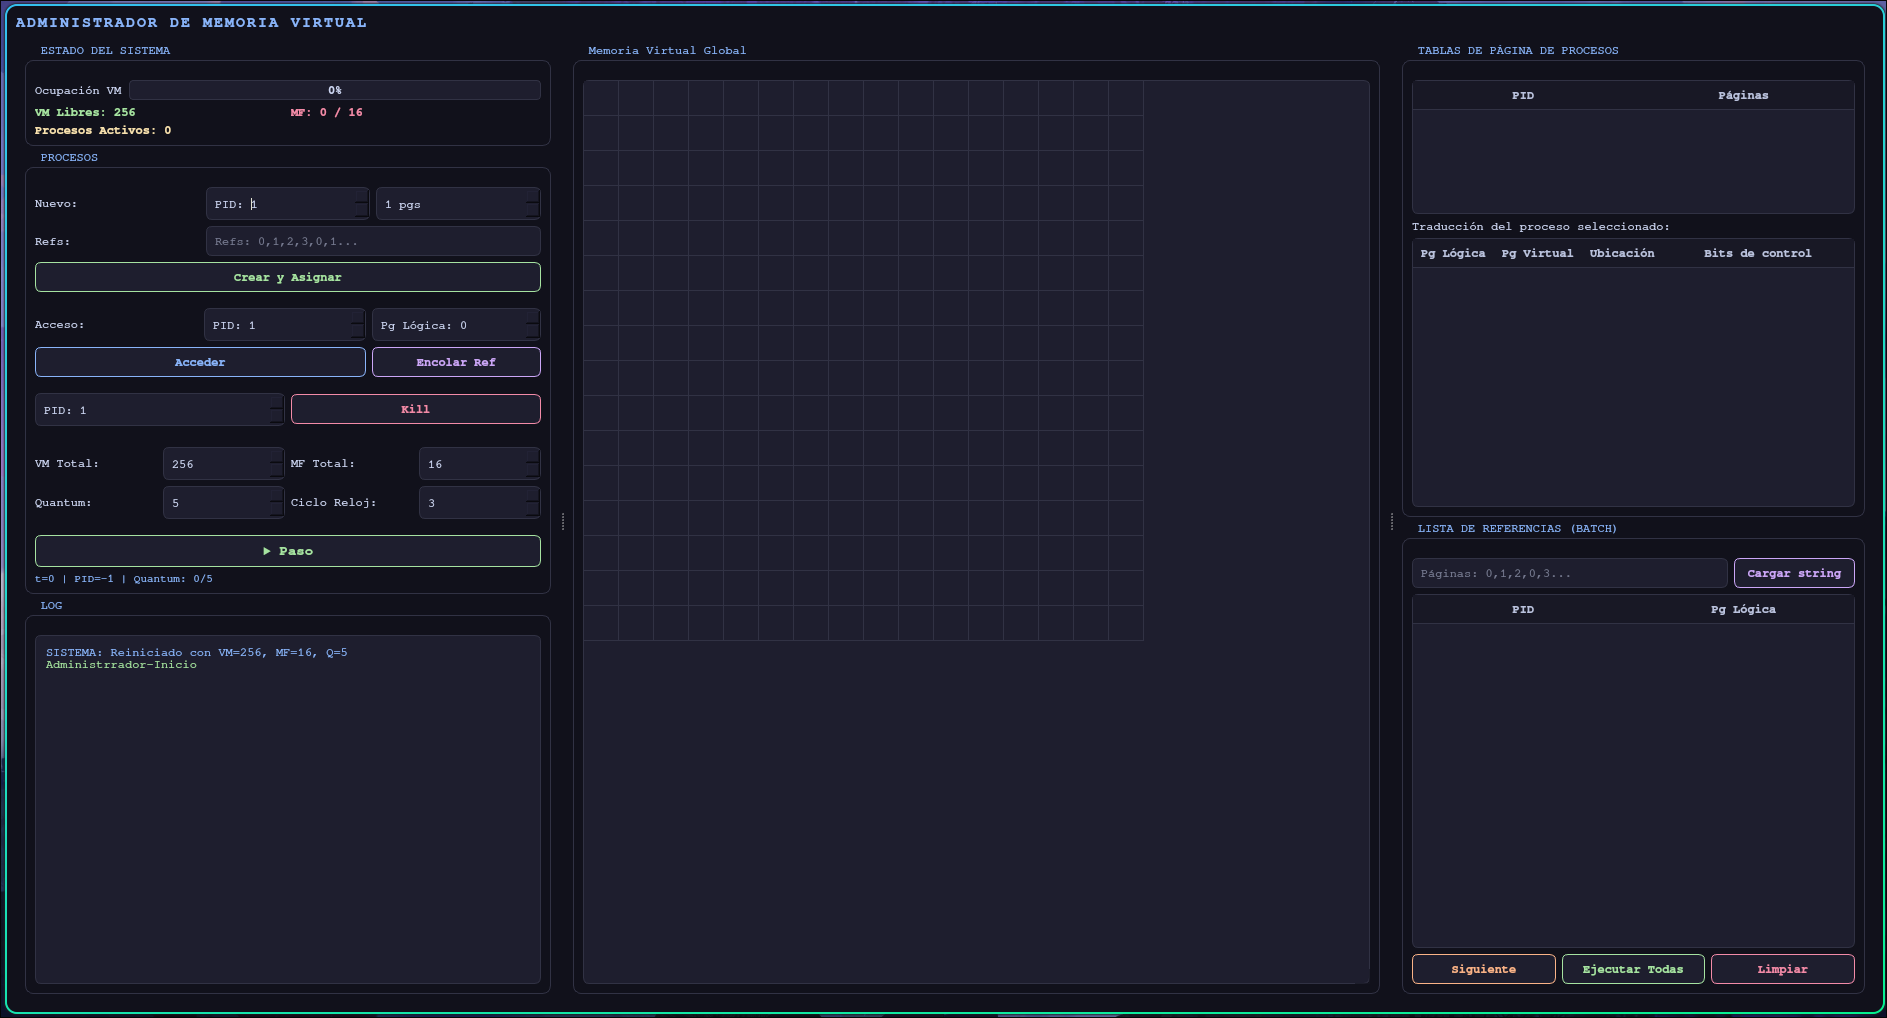
\includegraphics[width=\linewidth]{capturas/figura12.png}
\centering


\end{tcolorbox}
\captionof{figure}{Vista general de la aplicación MemManager GUI.}

La pantalla principal se divide en controles (izquierda), visualización de memoria global (centro) y
detalles específicos de proceso y tablas (derecha).

\subsubsection{Configuración Inicial}

\begin{tcolorbox}[screenshotbox={Sección de QSpinBox para Memoria Virtual, RAM y Quantum}]
\centering
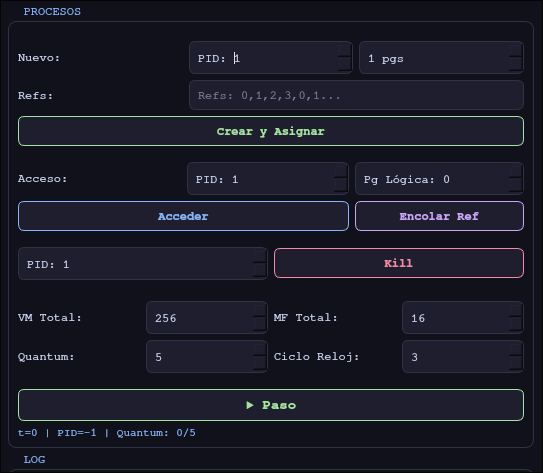
\includegraphics[width=\linewidth]{capturas/figura13.png}
\centering


\end{tcolorbox}
\captionof{figure}{Panel de configuración del simulador.}

Antes de agregar procesos, configure los parámetros del sistema operativo simulado.
Se recomienda mantener una proporción de al menos 4:1 entre VM y RAM para observar reemplazos.
\subsubsection{Crear un Proceso}

\begin{tcolorbox}[screenshotbox={Formulario de creación de proceso ingresando PID y Refs}]
\centering
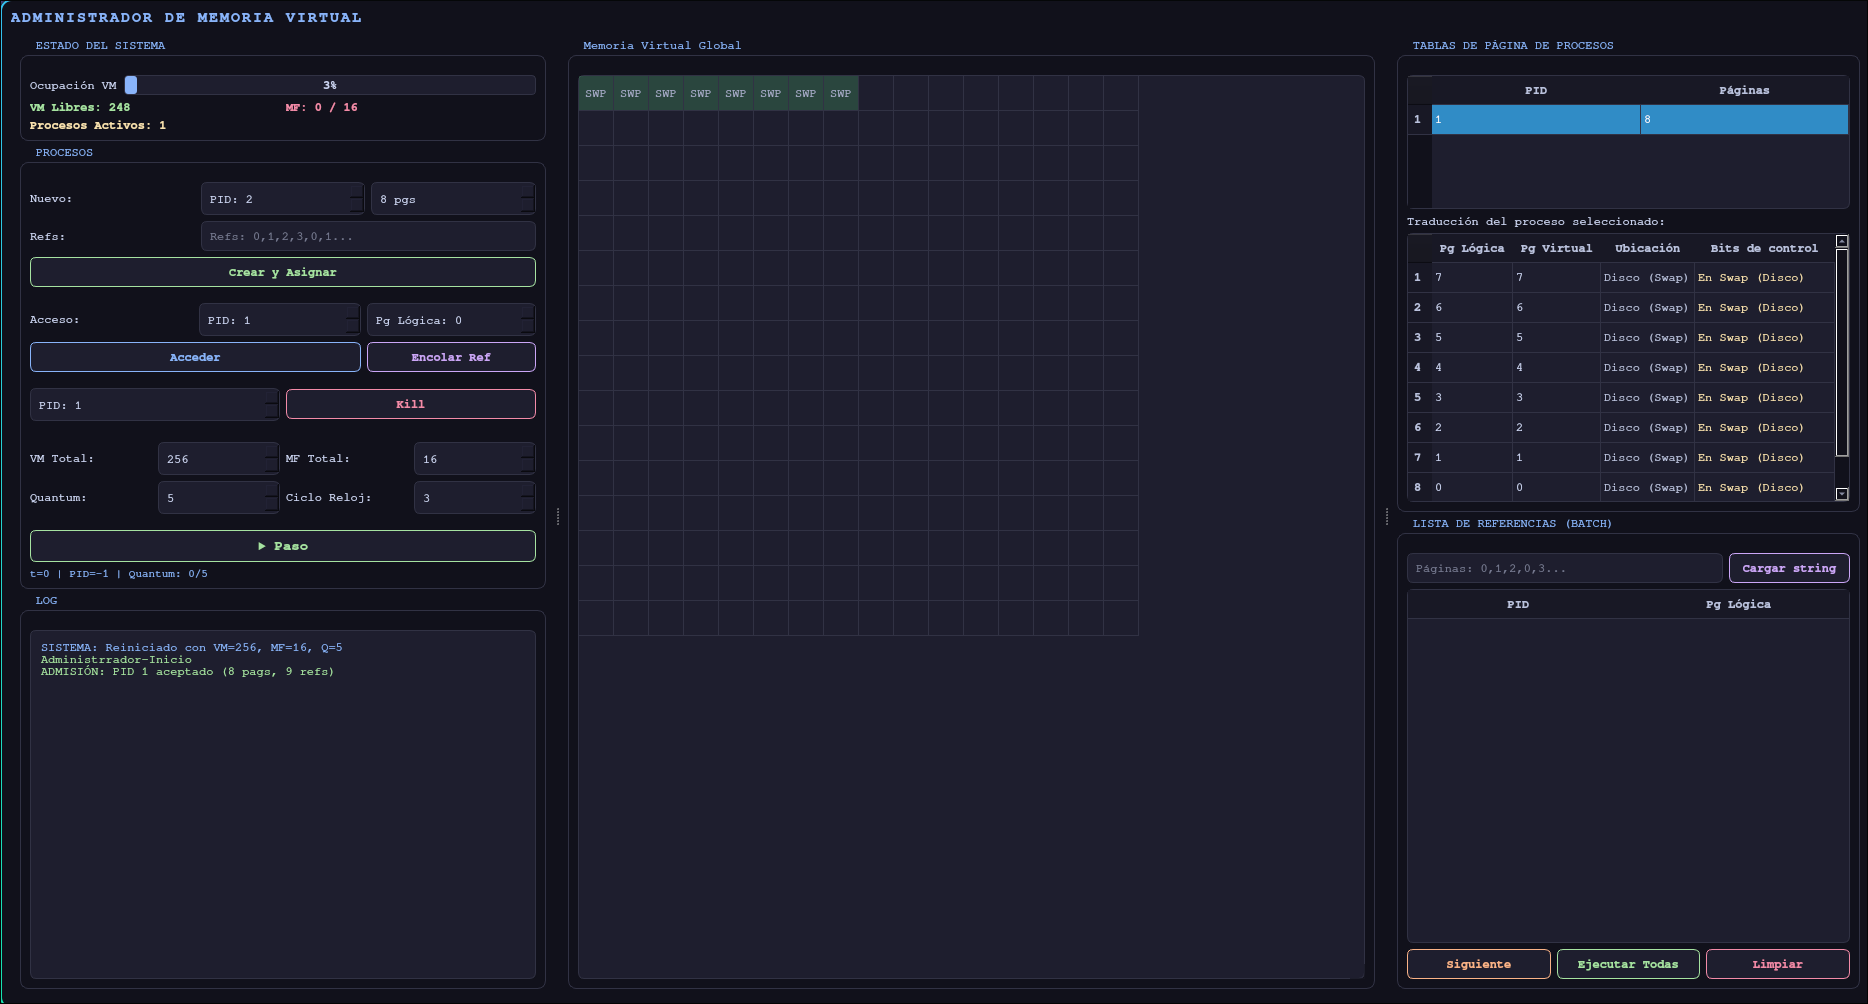
\includegraphics[width=\linewidth]{capturas/figura14.png}
\centering


\end{tcolorbox}
\captionof{figure}{Creación de un proceso interactivo.}

\begin{enumerate}
    \item Ingresar PID (ej. 1).
\item Ingresar número de páginas (ej. 8).
    \item Ingresar lista de referencias separada por comas (ej. 0,1,2,0,3,1,4,2,0).
\item Clic en "Crear y Asignar".
    \item Observar la cuadrícula de memoria virtual actualizarse con el color del proceso.
\end{enumerate}

\subsubsection{Ejecutar Paso a Paso}
\begin{tcolorbox}[screenshotbox={Botón de Paso y registro del Log (QTextEdit)}]
\centering
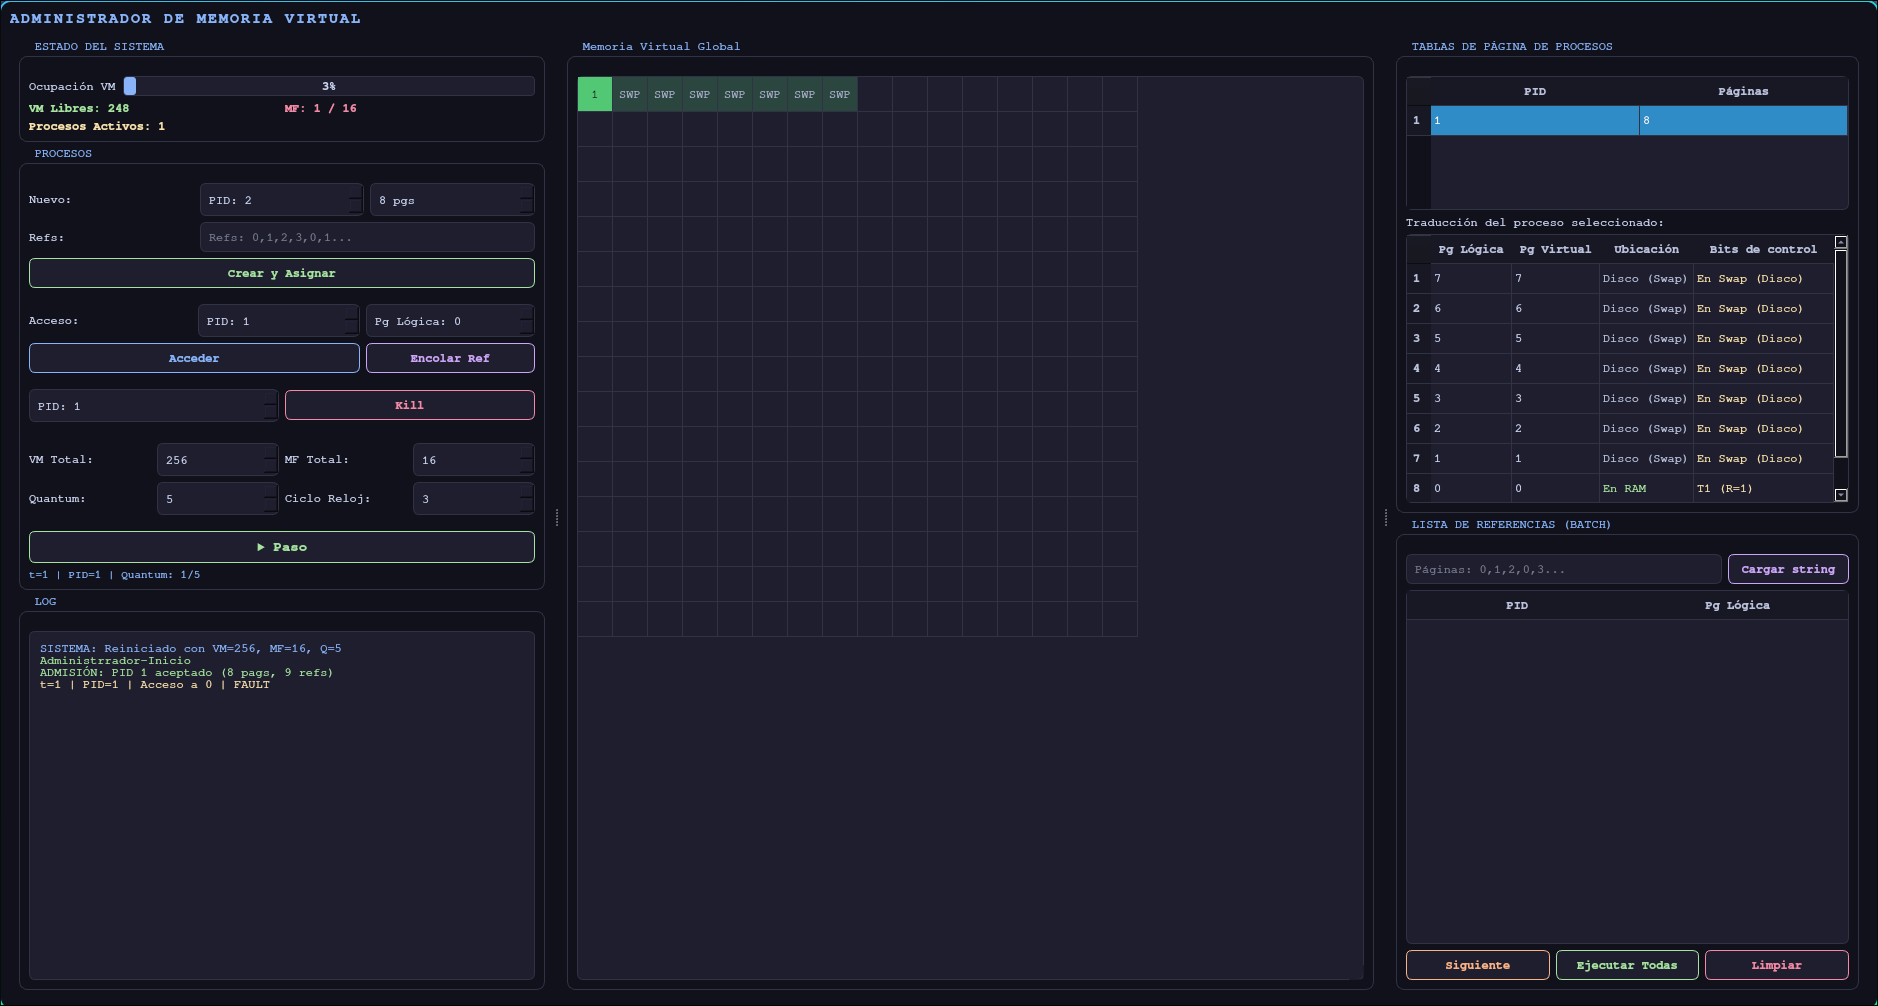
\includegraphics[width=\linewidth]{capturas/figura15.png}
\centering


\end{tcolorbox}
\captionof{figure}{Ejecución interactiva y bitácora.}

Presione el botón \textbf{$\blacktriangleright$ Paso} para avanzar el tiempo de CPU en 1 unidad.
El registro documentará si ocurrió un \textit{Hit} o un \textit{Fallo de Página}.
\subsubsection{Alerta de Fallo de Página}

\begin{tcolorbox}[screenshotbox={Cuadro de diálogo QMessageBox advirtiendo un Fallo Duro de Página}]
\centering
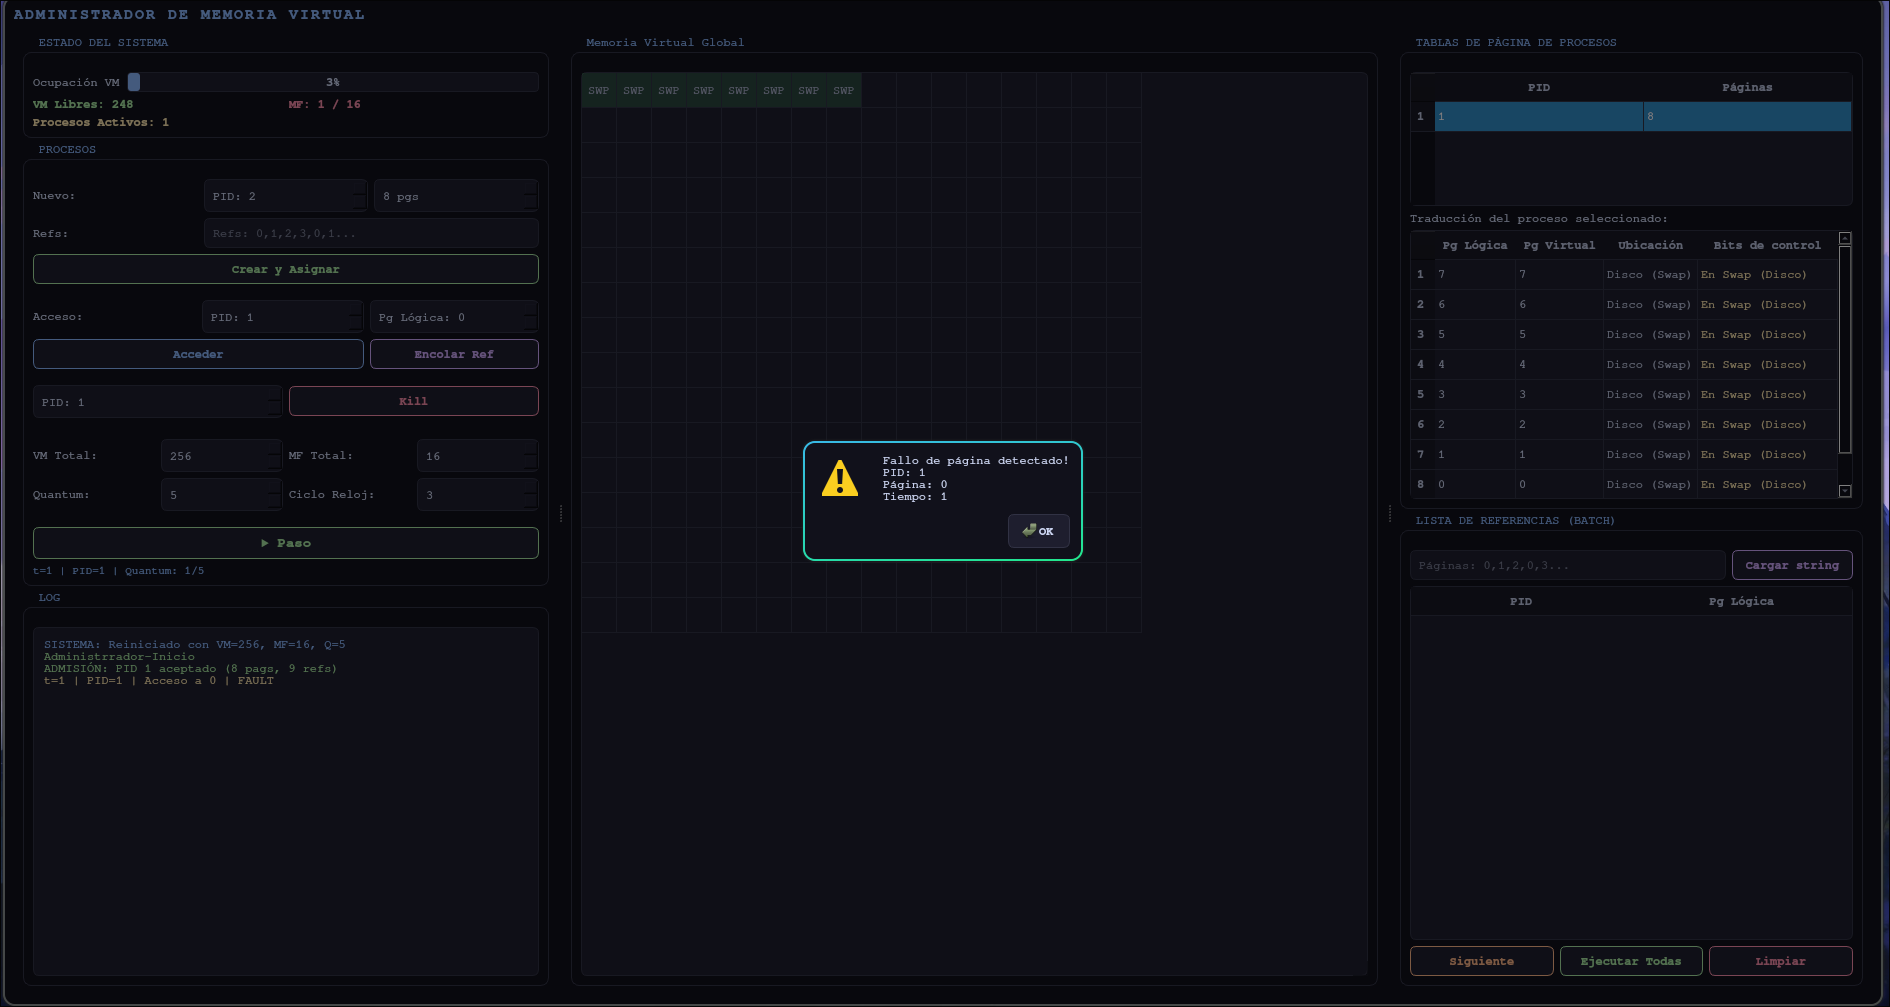
\includegraphics[width=\linewidth]{capturas/figura16.png}
\centering


\end{tcolorbox}
\captionof{figure}{Alerta interactiva del simulador.}

Cuando la RAM está llena y se requiere cargar una página nueva, el simulador pausa la ejecución y muestra esta advertencia, indicando qué página víctima ha sido elegida por el algoritmo de reemplazo CAR.
\subsubsection{Tabla de Páginas del Proceso}

\begin{tcolorbox}[screenshotbox={QTableWidget mostrando Páginas Lógicas, Globales, RAM/Disco y Bits}]
\centering
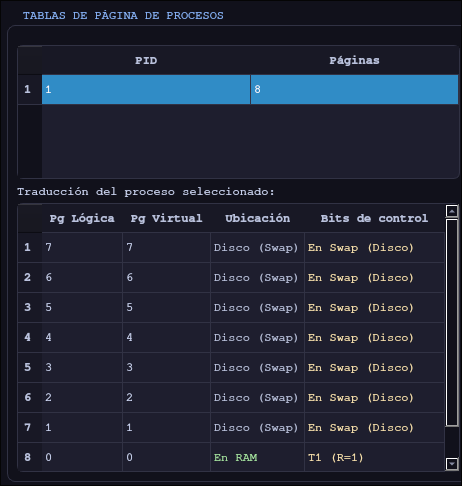
\includegraphics[width=\linewidth]{capturas/figura17.png}
\centering


\end{tcolorbox}
\captionof{figure}{Visor de la Tabla de Páginas.}

Seleccione un proceso en la lista superior derecha para inspeccionar su tabla de páginas.
Columnas visibles: Página Lógica, Página Virtual Global, Ubicación (RAM/Disco), y Bits de Control ($R$, Validez).
\subsubsection{Reporte Final}

\begin{tcolorbox}[screenshotbox={Dialog FinalReport mostrando tiempos y fallos del proceso terminado}]
\centering
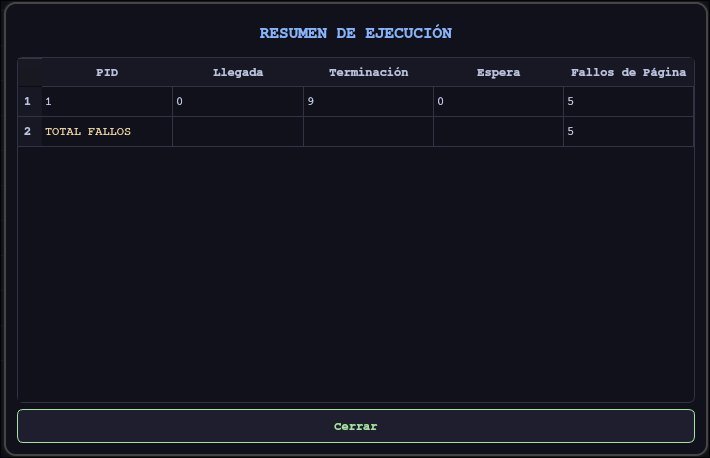
\includegraphics[width=\linewidth]{capturas/figura18.png}
\centering


\end{tcolorbox}
\captionof{figure}{Reporte de terminación.}

Métricas reportadas:
\begin{itemize}
    \item \textbf{Tiempo de Llegada}: Cuándo el proceso entró al sistema.
\item \textbf{Tiempo de Terminación}: Instante exacto en que procesó su última referencia.
\item \textbf{Tiempo de Espera}: Unidades de tiempo pasadas en la \texttt{readyQueue\_} sin CPU.
\item \textbf{Fallos de Página}: Total de penalizaciones de I/O por no hallar la página en RAM.
\end{itemize}

\subsection{Guía del Servidor y Cliente (Parte 2)}

\subsubsection{Iniciar el Servidor}
\begin{tcolorbox}[terminalbox, title={Terminal del Servidor}]
\begin{verbatim}
cd network
./memserver 9000
# Salida:
# [SERVER] Escuchando en puerto 9000
# [SERVER] Thread pool: 8 workers activos
# [SERVER] Dispatcher iniciado (quantum=5, ciclo=3)
\end{verbatim}
\end{tcolorbox}

\subsubsection{Enviar un Proceso desde un Cliente}
\begin{minipage}[t]{0.48\textwidth}
\begin{tcolorbox}[terminalbox, title={Terminal A (Nodo 1)}]
\begin{verbatim}
./memclient 127.0.0.1 9000 \
  1 8 0,1,2,0,3,1,4,2
# [OK] Proceso 1 registrado
# ... esperando resultado ...
# [DONE] PID=1
#   Tiempo fin: 13
#   Tiempo espera: 5
#   Fallos de página: 6
\end{verbatim}
\end{tcolorbox}
\end{minipage}\hfill
\begin{minipage}[t]{0.48\textwidth}
\begin{tcolorbox}[terminalbox, title={Terminal B (Nodo 2)}]
\begin{verbatim}
./memclient 127.0.0.1 9000 \
  2 6 3,4,3,0,1,4
# [OK] Proceso 2 registrado
# ... esperando resultado ...
# [DONE] PID=2
#   Tiempo fin: 18
#
 Tiempo espera: 7
#   Fallos de página: 4
\end{verbatim}
\end{tcolorbox}
\end{minipage}

\subsubsection{Monitorear el Servidor}
\begin{tcolorbox}[terminalbox, title={Terminal del Monitor}]
\begin{verbatim}
./memmonitor 127.0.0.1 9000 2000
\end{verbatim}
\end{tcolorbox}
Esto despliega la tabla Unicode en tiempo real que se actualiza cada 2 segundos.
Note que puede ejecutarse desde la misma máquina anfitrión (\texttt{localhost} / \texttt{127.0.0.1}) sin problemas, ya que el servidor atiende los sockets independientemente del origen IP.
\subsection{Interpretación de Resultados}

\begin{tcolorbox}[infobox, title={Entendiendo las Métricas}]
\begin{itemize}
    \item \textbf{Tiempo de terminación:} el instante (en referencias) en que el proceso completó toda su cadena de referencias.
\item \textbf{Tiempo de espera:} referencias que el proceso pasó en la cola listo, sin ejecutarse.
\item \textbf{Fallos de página:} cuántas veces una referencia no encontró la página en RAM y tuvo que traerla desde el área de swap.
\end{itemize}
\end{tcolorbox}

\begin{tcolorbox}[alertbox, title={Cuidado con el Thrashing}]
Un número alto de fallos de página combinado con tiempo de espera alto puede indicar \textit{thrashing}.
Considere aumentar el número de marcos de RAM (MF Total) o reducir el número de páginas por proceso.
\end{tcolorbox}

\subsection{Solución de Problemas}

\begin{table}[H]
\centering
\rowcolors{2}{catBlue!10}{white}
\begin{tabular}{|p{3.2cm}|p{4.5cm}|p{7.5cm}|}
\hline
\rowcolor{catBlue!40}
\textbf{Síntoma} & \textbf{Causa probable} & \textbf{Solución} \\
\hline
Cannot connect to server & Servidor no iniciado o puerto incorrecto & Verificar que \texttt{memserver} esté corriendo y el puerto coincida \\
\hline
ERR duplicate pid & PID ya registrado en el servidor & Usar un PID diferente \\
\hline
GUI no responde al paso & Dispatcher sin procesos en cola & Crear al menos un proceso antes de hacer clic en Paso \\
\hline
Ventana muy pequeña & Resolución menor a 1280x720 & Maximizar ventana o aumentar resolución \\
\hline
Segfault en acceso & Página lógica fuera del rango & Verificar que las referencias usen índices de 0 a numPages-1 \\
\hline
\end{tabular}
\caption{Solución de problemas comunes.}
\end{table}

\newpage
\section{Pruebas y Resultados}

\subsection{Metodología de Pruebas}
Las pruebas fueron diseñadas con cadenas de referencia deterministas.
Este enfoque aísla variables y permite evaluar comportamientos específicos:
\begin{itemize}
    \item \textbf{Alta Conflictividad}: Excede intencionalmente el límite de memoria para forzar thrashing.
\item \textbf{Localidad de Referencia}: Simula un conjunto de trabajo (working set) estable para probar si la política evita la penalización continua.
\end{itemize}

\subsection{Prueba 1 --- Alta Conflictividad (Thrashing)}
\textbf{Setup:} 4 marcos RAM, 3 procesos de 6 páginas, quantum = 4.
Cadenas de referencia (cada una barre todas sus páginas sin localidad):
\begin{itemize}
    \item \textbf{P1:} 0,1,2,3,4,5,0,1,2,3,4,5 (12 refs)
    \item \textbf{P2:} 0,1,2,3,4,5,0,1,2,3,4,5 (12 refs lógicas)
    \item \textbf{P3:} 0,2,4,1,3,5,0,2,4 (9 refs)
\end{itemize}

\begin{table}[H]
\centering
\rowcolors{2}{catBlue!10}{white}
\begin{tabular}{@{}lllllr@{}}
\toprule
\rowcolor{catBlue!40}
\textbf{PID} & \textbf{Llegada} & \textbf{Terminación} & \textbf{Espera} & \textbf{Fallos Pág.} & \textbf{Hit Rate} \\ \midrule
1 & 0 & 31 & 19 & 10 & 16.6\% \\
2 & 0 & 32 & 20 & 11 & 8.3\% \\
3 & 0 & 26 & 17 & 8 & 11.1\% \\ \bottomrule
\end{tabular}
\caption{Resultados bajo condiciones de Thrashing.}
\end{table}

\begin{figure}[H]
\centering
\begin{tcolorbox}[colback=gray!10, colframe=gray!30, arc=4pt]
\centering
\textbf{Gráfico: Fallos de página por proceso (Prueba 1)}\\[0.5em]
\rule{\textwidth}{0.4pt}\\[0.5em]
P1: 10 fallos \hfill P2: 11 fallos \hfill P3: 8 fallos
\end{tcolorbox}
\caption{Fallos de página por proceso (Prueba 1).}
\end{figure}

Análisis: Sin localidad, ningún algoritmo de reemplazo sobrevive sin un alto número de fallos.
Sin embargo, los historiales fantasma de HybridPolicy (CAR) mitigaron el desastre al promover tempranamente las páginas de T1 a T2 una vez readquiridas, un comportamiento superior al de un LRU estricto que hubiera penalizado repetidamente el mismo conjunto.
\subsection{Prueba 2 --- Localidad de Referencia}
\textbf{Setup:} 8 marcos RAM, 3 procesos, quantum = 5.
Cadenas de referencia (fuerte localidad):
\begin{itemize}
    \item \textbf{P1:} 0,1,2,0,1,2,0,1,2,0,1,2 (12 refs)
    \item \textbf{P2:} 3,4,3,4,3,4,3,4 (8 refs)
    \item \textbf{P3:} 0,1,2,3,0,1,2,3,0 (9 refs)
\end{itemize}

\begin{table}[H]
\centering
\rowcolors{2}{catBlue!10}{white}
\begin{tabular}{@{}lllllr@{}}
\toprule
\rowcolor{catBlue!40}
\textbf{PID} & \textbf{Llegada} & \textbf{Terminación} & \textbf{Espera} & \textbf{Fallos Pág.} & \textbf{Hit Rate} \\ \midrule
1 & 0 & 24 & 12 & 3 & 75.0\% \\
2 & 0 & 16 & 8 & 2 & 75.0\% \\
3 & 0 & 29 & 20 & 4 & 55.5\% \\ \bottomrule
\end{tabular}
\caption{Resultados con alta localidad de referencia.}
\end{table}

\begin{figure}[H]
\centering
\begin{tcolorbox}[colback=gray!10, colframe=gray!30, arc=4pt]
\centering
\textbf{Comparación de fallos de página}\\[0.5em]
\rule{\textwidth}{0.4pt}\\[0.5em]
Prueba 1 (Thrashing): P1=10, P2=11, P3=8\\[0.2em]
Prueba 2 (Localidad): P1=3, P2=2, P3=4
\end{tcolorbox}
\caption{Comparación de fallos de página entre escenarios.}
\end{figure}

\subsection{Prueba 3 --- Concurrencia (Parte 2)}
Se lanzaron 5 clientes con una ráfaga inicial.
\begin{table}[H]
\centering
\rowcolors{2}{catBlue!10}{white}
\begin{tabular}{@{}llrrr@{}}
\toprule
\rowcolor{catBlue!40}
$t$ \textbf{(ms)} & \textbf{Evento} & \textbf{Conexiones Activas} & \textbf{Workers} & \textbf{Pendientes} \\ \midrule
0 & Servidor Inicia & 0 & 0 & 0 \\
10 & 5 CREATE simultáneos & 5 & 5 (4 max pool) & 1 \\
20 & Procesamiento de Admisión & 5 & 4 & 0 \\
25 & Dispatcher encolando & 5 & 0 & 0 \\
500 & DONE P1 y P2 & 3 & 0 & 0 \\
1200 & DONE restantes & 0 & 0 & 0 \\ \bottomrule
\end{tabular}
\caption{Métricas del monitor durante un ataque en ráfaga (burst).}
\end{table}
El pool absorbió la carga sin crear 5 hilos de sistema.
La tarea "pendiente" fue despachada tan pronto como el worker 1 finalizó la admisión del primer cliente.
\subsection{Análisis Comparativo Adicional}

\begin{figure}[H]
\centering
\begin{tcolorbox}[colback=gray!10, colframe=gray!30, arc=4pt]
\centering
\textbf{Comparación de Tiempos de Espera ($T_w$)}\\[0.5em]
\rule{\textwidth}{0.4pt}\\[0.5em]
Prueba 1 (Thrashing): P1=19, P2=20, P3=17\\[0.2em]
Prueba 2 (Localidad): P1=12, P2=8, P3=20
\end{tcolorbox}
\caption{Comparación de Tiempos de Espera.}
\end{figure}

\newpage
\section{Discusión}

El desarrollo de este simulador arrojó a la luz varios compromisos y decisiones técnicas profundas.
Una de las más destacadas fue la implementación de CAR (Clock with Adaptive Replacement) sobre un LRU tradicional.
En un simulador, mantener una lista exacta de LRU es trivial porque no existen las restricciones del hardware real;
sin embargo, implementar CAR ofrece una aproximación pedagógica invaluable al diseño de sistemas operativos modernos (como Linux, que usa listas activas/inactivas).
Observar cómo el parámetro dinámico $p$ de la \texttt{HybridPolicy} se ajusta en base a los historiales fantasma B1 y B2 provee un entendimiento visual del equilibrio entre recencia y frecuencia que ninguna teoría en papel puede igualar.
Un desafío inherente fue la representación de las cadenas de referencia.
A diferencia de un sistema real donde las referencias de memoria son generadas en ráfagas densas de millones por segundo, capturables mediante herramientas como Valgrind o Intel PIN, este simulador opera bajo un modelo determinista manual.
Esto introduce una limitación: los patrones de localidad en el simulador son extremadamente cortos, requiriendo adaptar artificialmente parámetros como la constante \texttt{REFS\_PER\_CYCLE} para que el algoritmo CAR pueda mostrar su comportamiento a una escala observable en la GUI.
Por otro lado, la incorporación del patrón Thread Pool revolucionó la arquitectura del simulador de una aplicación aislada a un verdadero servidor concurrente.
Mientras que el enfoque ingenuo (un \texttt{std::thread} por socket de cliente) era adecuado para un prototipo, el pool garantizó un consumo de recursos acotado y protegió contra sobrecargas masivas de red, un concepto fundamental en Sistemas Operativos.
No obstante, el sistema actual no constituye una arquitectura verdaderamente distribuida: carece de tolerancia a fallos, no hay replicación del MemoryManager, y todos los procesos compiten finalmente por el mismo mutex monolítico \texttt{dispatcherMutex\_}.
En un kernel real, el equivalente a esta protección serían múltiples \textit{spinlocks} de grano fino, estructuras \textit{RCU} (Read-Copy-Update), manipulaciones atómicas de las entradas de la tabla de páginas y operaciones IPI (Inter-Processor Interrupt) para invalidaciones remotas de la TLB (\textit{TLB shootdown}).
Nuestro simulador omite esta complejidad en favor de una sincronización macroscópica que garantiza consistencia sin comprometer el propósito didáctico.
Finalmente, el factor del quantum en el \texttt{Dispatcher} demostró un efecto esperado pero dramático.
Un quantum pequeño mejoró la equidad entre clientes interactivos en las pruebas de red, pero generó reportes con mayores retrasos de retorno (turnaround) debido a los cambios de contexto simulados.
Un quantum grande penalizó severamente a los clientes cuyas solicitudes requerían pocas referencias a memoria.
Esta observación empírica valida por completo la teoría del planificador Round Robin abordada en el curso.
Como trabajo futuro, integrar una visualización en tiempo real de cómo las páginas saltan de T1 a T2 y eventualmente a los historiales fantasma enriquecería aún más el valor académico del proyecto.
\newpage
\section{Conclusiones}

Este proyecto ha culminado exitosamente en un producto bifurcado altamente funcional: un simulador pedagógico visual de administración de memoria (GUI) y un servidor de procesamiento masivo tolerante a concurrencia (Red).
Se demostró satisfactoriamente el mapeo entre espacio virtual y físico, los mecanismos para resolver fallos de página y el despacho de la CPU mediante Round Robin.
La elección de implementar CAR desde cero demostró ser un ejercicio de rigor técnico.
Demandó un entendimiento profundo no solo del clásico mecanismo de Reloj, sino del mecanismo de recolección de historiales de la arquitectura ARC de IBM.
Esto elevó el techo técnico del equipo, pasando de meros consumidores de la teoría de sistemas operativos a implementadores funcionales.
El éxito del servidor bajo condiciones de estrés demostró además que las primitivas de sincronización modernas en C++20 son herramientas maduras y formidables para desarrollar software a nivel de sistemas.
\begin{itemize}
    \item \textbf{Razo Montañez Gael Askary:} "Este proyecto consolidó mi comprensión de la gestión de memoria. Programar el Thread Pool me forzó a enfrentar problemas reales de concurrencia y a utilizar abstracciones modernas como \texttt{std::condition\_variable}, entendiendo por qué los servidores reales no pueden darse el lujo de lanzar hilos sin control."
    \item \textbf{Ángel Hernández González:} "Implementar la lógica del Dispatcher junto con la política de reemplazo desmitificó el término 'fallo de página' para mí. Ver el efecto cascada de un algoritmo de reemplazo deficiente en las pruebas de estrés me hizo apreciar los desafíos inherentes al diseño del kernel de un sistema operativo."
    \item \textbf{José Gabriel Hernández Mejía:} "La arquitectura del simulador y su acoplamiento con la interfaz gráfica presentó un desafío fascinante de diseño de software. Asegurarse de que el estado interno del Memory Manager se reflejara con precisión y sin bloqueos en la GUI solidificó mi comprensión sobre el paradigma Modelo-Vista-Controlador en C++."
\end{itemize}
Como vías de investigación futuras, proponemos extender la arquitectura hacia un sistema distribuido real, permitiendo nodos esclavos ejecutando sus propios MemoryManagers.
Así mismo, la capacidad de ingerir trazas de memoria reales (e.g. vía \texttt{/proc/pid/smaps}) acercaría al simulador a los estándares analíticos industriales.
\newpage
\section{Referencias}

\begin{thebibliography}{99}

\bibitem{silberschatz2018}
Silberschatz, A., Galvin, P. B., \& Gagne, G. (2018). \textit{Operating System Concepts} (10.ª ed.). Wiley.
\bibitem{tanenbaum2014}
Tanenbaum, A. S., \& Bos, H. (2014). \textit{Modern Operating Systems} (4.ª ed.). Pearson.

\bibitem{bansal2004}
Bansal, S., \& Modha, D. S. (2004).
CAR: Clock with Adaptive Replacement. \textit{Proceedings of the 3rd USENIX Conference on File and Storage Technologies (FAST '04)}, 187--200.
\bibitem{megiddo2003}
Megiddo, N., \& Modha, D. S. (2003). ARC: A Self-Tuning, Low Overhead Replacement Cache. \textit{FAST '03}, 115--130.

\bibitem{qt2024}
Qt Project. (2024).
\textit{Qt 6 Documentation}. Recuperado de \url{https://doc.qt.io/qt-6/}

\bibitem{stroustrup2013}
Stroustrup, B. (2013). \textit{The C++ Programming Language} (4.ª ed.). Addison-Wesley.
\bibitem{stevens2013}
Stevens, W. R., \& Rago, S. A. (2013). \textit{Advanced Programming in the UNIX Environment} (3.ª ed.). Addison-Wesley.

\bibitem{williams2019}
Williams, A. (2019).
\textit{C++ Concurrency in Action} (2.ª ed.). Manning Publications.

\bibitem{denning1968}
Denning, P. J. (1968). Thrashing: Its Causes and Prevention.
\textit{Proceedings of the AFIPS Fall Joint Computer Conference}, 915--922.

\bibitem{intel2023}
Intel Corporation. (2023).
\textit{Intel® 64 and IA-32 Architectures Software Developer's Manual}, Vol. 3A: System Programming Guide.

\end{thebibliography}

\end{document}
